\documentclass[11pt,letterpaper]{article}

% Compile from the folder containing this file.
% This path works in template/ and in sibling course folders.
% Shared formatting for course notes. Loaded by each course's main.tex.
\usepackage[T1]{fontenc}
\usepackage[utf8]{inputenc}
\usepackage{lmodern}
\linespread{1.15}
\usepackage[margin=1in]{geometry}
\usepackage{amsmath,amssymb,amsthm}
\usepackage{mathtools}
\usepackage{graphicx}
\usepackage{booktabs}
\usepackage{enumitem}
\usepackage{xcolor}
\usepackage{hyperref}
\usepackage{tikz}
\usetikzlibrary{decorations.pathreplacing,positioning}
\usepackage{xparse}
\usepackage{etoolbox}

\hypersetup{colorlinks=true,linkcolor=blue!50!black,urlcolor=blue!50!black}
\setlength{\parindent}{0pt}
\setlength{\parskip}{0.5em}
\setlist{nosep}

% Unnumbered section headings: entries show as "Week 1", not "1 Week 1",
% both in the body and in the table of contents.
\setcounter{secnumdepth}{0}

% Each \section (i.e. each week's entry) starts on its own new page. The
% \newpage that used to follow \tableofcontents in each course's main.tex
% is redundant now and has been removed, so week 1 isn't pushed to a blank
% page by this.
\pretocmd{\section}{\newpage}{}{\errmessage{Failed to patch \string\section}}

% Tracks whether \section was the most recent sectioning/lecture command,
% so a \newlecture immediately following a \section (the usual "week's
% first lecture" case) doesn't also throw in its own \newpage, which would
% otherwise leave a blank page between the two. Set true by \section, and
% cleared by \newlecture whether or not it was true, so it only fires for
% a \newlecture that directly follows a \section (nothing else in between).
\newbool{newlecture@justsection}
\pretocmd{\section}{\booltrue{newlecture@justsection}}{}{\errmessage{Failed to patch \string\section}}

% Custom head format: bold, unparenthesized title, with a \quad gap after
% the number (e.g. "Theorem 3.2  Distribution" instead of "Theorem 3.2
% (Distribution)."), reusing amsthm's usual spacing/punctuation otherwise.
% When a title is given, the body text starts on its own new line below the
% head instead of running inline after it; untitled (auto-numbered-only)
% instances stay inline as usual. Body text is upright (not italic) for all
% six environments. Two variants share this head format but differ in
% end-of-head punctuation: theorem/lemma/proposition/exercise keep a
% trailing period, definition/example drop it (no period after the title).
\makeatletter
\newcommand{\thmpunct}{.}
\newtheoremstyle{boldhead}{}{}{\normalfont}{}{\bfseries}{\thmpunct}{5pt plus 1pt minus 1pt}%
    {\thmname{#1}\thmnumber{\@ifnotempty{#1}{ }#2}\thmnote{\@ifnotempty{#3}{\quad#3}}%
     \@ifnotempty{#3}{\def\thmheadnl{\newline}\thm@headsep\z@skip}{}}
\newtheoremstyle{boldheadnp}{}{}{\normalfont}{}{\bfseries}{}{5pt plus 1pt minus 1pt}%
    {\thmname{#1}\thmnumber{\@ifnotempty{#1}{ }#2}\thmnote{\@ifnotempty{#3}{\quad#3}}%
     \@ifnotempty{#3}{\def\thmheadnl{\newline}\thm@headsep\z@skip}{}}
\makeatother

\theoremstyle{boldhead}
\newtheorem{theorem}{Theorem}
\newtheorem{lemma}[theorem]{Lemma}
\newtheorem{proposition}[theorem]{Proposition}
\newtheorem{corollary}[theorem]{Corollary}
\newtheorem{exercise}[theorem]{Exercise}
\theoremstyle{boldheadnp}
\newtheorem{definition}[theorem]{Def.}
\newtheorem{example}[theorem]{Example}
\theoremstyle{remark}
\newtheorem*{remark}{Remark}

% \begin{theorem}[Title][2.7]: both optional arguments are new on top of
% the environments' usual single bracket. The first argument still behaves
% exactly like plain amsthm's optional title (existing notes using
% \begin{example}[Some Name] etc. are unaffected). The second argument, if
% given, overrides the displayed number (e.g. to match a textbook's own
% numbering) instead of the shared theorem counter's automatic value; the
% counter itself still advances normally, so later auto-numbered
% environments are unaffected too.
\newcommand{\addtitleandnumber}[1]{%
    \csletcs{#1orig}{#1}%
    \csletcs{end#1orig}{end#1}%
    \RenewDocumentEnvironment{#1}{o o}{%
        \IfValueT{##2}{\ifblank{##2}{}{\renewcommand{\thetheorem}{##2}}}%
        \IfValueTF{##1}{\ifblank{##1}{\csname#1orig\endcsname}{\csname#1orig\endcsname[##1]}}{\csname#1orig\endcsname}%
    }{\csname end#1orig\endcsname}%
}
\addtitleandnumber{theorem}
\addtitleandnumber{lemma}
\addtitleandnumber{proposition}
\addtitleandnumber{corollary}
\addtitleandnumber{definition}
\addtitleandnumber{example}
\addtitleandnumber{exercise}

% Common mathematical notation.
\newcommand{\R}{\mathbb{R}}
\newcommand{\N}{\mathbb{N}}
\newcommand{\Z}{\mathbb{Z}}
\newcommand{\E}{\mathbb{E}}
\newcommand{\Prob}{\mathbb{P}}
\DeclareMathOperator{\Var}{Var}
\DeclareMathOperator{\Cov}{Cov}

% \newlecture[title][date]: bold, centered marker for the start of a new
% lecture. Both arguments are optional. Numbering runs continuously across
% the whole document (i.e. across all weeks' entries, not reset per
% \section), so the Nth \newlecture in the course is always "Lecture N".
% Each lecture starts on its own new page, except when it directly follows
% a \section heading (which already started a new page of its own), so the
% two stay together instead of leaving a blank page in between.
\newcounter{lecture}
\renewcommand{\thelecture}{\arabic{lecture}}
% Set \lecturetoctrue in a course's main.tex to list each lecture as a
% top-level table-of-contents entry ("Lecture N: title", or the date when
% untitled), with \subsection headings nested beneath it.
\newif\iflecturetoc
\NewDocumentCommand{\newlecture}{o o}{%
    \stepcounter{lecture}%
    \ifbool{newlecture@justsection}{}{\newpage}%
    \boolfalse{newlecture@justsection}%
    \iflecturetoc
        \phantomsection
        \addcontentsline{toc}{section}{Lecture \thelecture\IfValueTF{#1}{\ifblank{#1}{\IfValueT{#2}{\ifblank{#2}{}{ (#2)}}}{: #1}}{\IfValueT{#2}{\ifblank{#2}{}{ (#2)}}}}%
    \fi
    \par\vspace{1em}
    \begin{center}
        \textbf{\Large Lecture \thelecture\IfValueT{#1}{: #1}}\\[2pt]
        \IfValueT{#2}{\normalsize #2}
    \end{center}
    \vspace{0.5em}%
}

% Handwritten-note-style helpers: red definition labels, blue margin
% annotations, yellow highlights, underlined mini-headers.
\newcommand{\deflabel}[2]{\par\noindent{\color{red!70!black}\textbf{Def #1}}\quad\textbf{#2}\par\nobreak}
\newcommand{\exlabel}[2]{\par\noindent\textbf{Example #1}\quad\textbf{#2}\par\nobreak}
\newcommand{\heading}[1]{\par\noindent{\color{red!70!black}\textbf{#1}}\par}
\newcommand{\header}[1]{\par\vspace{0.5em}\noindent\textbf{#1}\par\vspace{-0.2em}}
\newcommand{\aside}[1]{\ifmmode{\color{blue!55!black}\text{\itshape #1}}\else{\color{blue!55!black}\itshape #1}\fi}
\newcommand{\hly}[1]{\colorbox{yellow!55}{$#1$}}
\newcommand{\hlt}[1]{\colorbox{yellow!55}{#1}}
% \boldmath makes any math the argument switches into (e.g. \rb{$r$}) use
% the bold math version automatically, so callers don't need to manually
% wrap math content in \boldsymbol{}.
\newcommand{\rb}[1]{{\color{red!70!black}\boldmath\textbf{#1}}}
\renewcommand{\b}[1]{\textbf{#1}}
\definecolor{navy}{RGB}{0,32,96}
\newcommand{\dbb}[1]{{\color{navy}\textbf{#1}}}
\newcommand{\db}[1]{{\color{navy}#1}}

% Wider padding inside \boxed{} equations (default \fboxsep is 3pt).
% Scoped to \boxed only, so \colorbox highlights (e.g. \hly) are unaffected.
\let\oldboxed\boxed
\renewcommand{\boxed}[1]{{\setlength{\fboxsep}{10pt}\oldboxed{#1}}}


% Replace these details for each course.
\newcommand{\coursecode}{STA347}
\newcommand{\coursename}{Probability}
\newcommand{\term}{Fall 2026}
\newcommand{\studentname}{Bonnie Zhuang}

\title{\coursecode{} --- \coursename\\[0.5em]\large Course Notes}
\author{\studentname}
\date{\term}

% STA347-only override: the defined term in \deflabel is red too
% (shared default keeps it black), matching "Def #" already being red.
\renewcommand{\deflabel}[2]{\par\noindent{\color{red!70!black}\textbf{Def #1}}\quad\textbf{\color{red!70!black}#2}\par\nobreak}

% STA347-only override: no trailing period after theorem/lemma/etc. titles.
\renewcommand{\thmpunct}{}

\lecturetoctrue

% STA347-only: clickable midterm-required theorems.
% \req{key} at a theorem drops an anchor; \rl{key}{text} links to it;
% \reqtoc{key}{text}, placed at the theorem, adds a TOC line + PDF bookmark
% under that theorem's own lecture.
\usepackage{bookmark}
\newcommand{\req}[1]{\hypertarget{req:#1}{}\label{req:#1}}
% Required (with proof) -> red bold heading + red "Proof";
% required, no proof -> blue bold heading. Body text stays normal.
\makeatletter
\newcommand{\reqhead}[1]{%
    \let\reqoldboldhead\th@boldhead
    \def\th@boldhead{\reqoldboldhead\thm@headfont{\bfseries\color{#1}}}%
    \let\reqoldboldheadnp\th@boldheadnp
    \def\th@boldheadnp{\reqoldboldheadnp\thm@headfont{\bfseries\color{#1}}}%
    % clicking the heading jumps to the Lec 12 required list
    \hypersetup{linkcolor=#1}%
    \let\reqoldthhead\th@boldhead
    \def\th@boldhead{\reqoldthhead\reqlinkhead}%
    \let\reqoldthheadnp\th@boldheadnp
    \def\th@boldheadnp{\reqoldthheadnp\reqlinkhead}}
\newcommand{\reqprefix}{}% "*" on required headings
\newcommand{\reqlinkhead}{%
    \let\reqoldthmhead\thmhead
    \def\thmhead##1##2##3{\@ifempty{##3}%
        {\reqoldthmhead{\hyperlink{req:list}{\reqprefix##1}}{\hyperlink{req:list}{##2}}{}}%
        {\reqoldthmhead{\hyperlink{req:list}{\reqprefix##1}}{\hyperlink{req:list}{##2}}{\hyperlink{req:list}{##3}}}}}
\makeatother
\newenvironment{reqproof}{\renewcommand{\reqprefix}{*}\reqhead{red!70!black}\renewcommand{\proofname}{\textcolor{red!70!black}{\bfseries Proof}}}{}
\newenvironment{reqnoproof}{\renewcommand{\reqprefix}{*}\reqhead{blue!60!black}}{}
\newcommand{\rl}[2]{\hyperref[req:#1]{#2}}
\newcommand{\reqtoc}[2]{%
    \addtocontents{toc}{\protect\contentsline{subsubsection}{#2}{\protect\pageref{req:#1}}{req:#1}}%
    \bookmark[dest=req:#1,level=2]{#2}}

% STA347-only: group lectures by chapter in the TOC / PDF outline.
% \chapterentry{title} goes right before a lecture's \input; it lands on the
% lecture's own page (no extra page break, \newlecture skips its \newpage).
\makeatletter
\newcommand{\chapterentry}[1]{\clearpage\phantomsection\addcontentsline{toc}{part}{#1}\booltrue{newlecture@justsection}}
\makeatother

\begin{document}
\maketitle
\tableofcontents

% Add one input per lecture, in the order you want them to appear.
\chapterentry{Chapter 1: Set Theory Fundamentals}
% !TeX root = ../main.tex

\newlecture[Set Theory Fundamentals][Sep 8, 2026]

``Probability = Set Theory + Measure''

\begin{enumerate}
    \item \textbf{Basic Set Operations}
    \\ Union, Intersect, Complement, \dots
    \\ $A\cup B,\ A\cap B,\ A^C, \dots$

    \item \deflabel{1.1.1}{Convergence of Real-Valued Sequences}
    \begin{quote}
        A sequence $(x_n)_{n=1}^\infty \subseteq \R$ converges to $x$ if
        \[\forall \varepsilon>0,\ \exists N \in \N \text{ s.t. } n>N \Rightarrow \left\lvert x_n-x\right\rvert < \varepsilon.\]
    \end{quote}
    $x_n \to x$ \text{converge to $x$?}
    \\ \text{Pick $\varepsilon$ (how close $x_n$ is to the target).}
    \\ For any $\varepsilon$ picked, can find $N$, such that $n>N$, $\left\lvert x_n-x\right\rvert < \varepsilon$.
    \\ e.g. $x_n = \dfrac{1}{n} \to 0$

    \item \deflabel{1.1.2}{Functional Convergence Pointwisely}
    \begin{quote}
        A sequence $(f_n)_{n=1}^\infty \subseteq \R^X$ converges pointwise to $f$ \text{(target $f$)} if
        \[\forall \varepsilon>0,\ \forall x \in X,\ \exists N_x \in \N \text{ s.t. } n>N_x \Rightarrow \left\lvert f_n(x)-f(x)\right\rvert < \varepsilon.\]
    \end{quote}
    $f_1,\dots,f_n,\dots$ --- \text{sequence of functions}
    \\ $f$ --- \text{target function}
    \\ For any $\varepsilon$ and $x$, can find $N_x$ s.t. $n>N_x$, $\left\lvert f_n(x)-f(x)\right\rvert < \varepsilon$.
    \\ $f_1(2), f_2(2), \dots, f_n(2), \dots \to f(2)$ --- \text{for every $x$, there is a corresponding $N_x$.}

    \item \deflabel{1.1.3}{Functional Convergence Uniformly}
    \begin{quote}
        A sequence $(f_n)_{n=1}^\infty \subseteq \R^X$ converges uniformly to $f$ if
        \[\forall \varepsilon>0,\ \hly{\exists N \in \N} \quad \forall x \in X,\ n>N \Rightarrow \left\lvert f_n(x)-f(x)\right\rvert < \varepsilon.\]
    \end{quote}
    \text{That works for all $x \in X$ --- need a common threshold $N$ for uniform convergence.}
\end{enumerate}

\heading{Key difference:}
For pointwise convergence, you need to have $x$ specified first, then there is a threshold $N_x$ corresponding to each $x$.
\\ For uniform convergence, you need a common threshold $N$ that works for all $x \in X$.

\begin{example}
    \[f_n(x) = \frac{x}{n+x}, \quad x\geq 0\]
    Then for any fixed value $x$, as $n\to\infty$, $f_n(x)\to 0$:
    \\ $x=1$: $f_n(1) = \dfrac{1}{n+1} \to 0$ as $n\to\infty$.
    \\ $x=2$: $f_n(2) = \dfrac{2}{n+2} \to 0$ as $n\to\infty$.
    \[\therefore f_n(x) \xrightarrow{\text{pointwise}} 0\]

    However, $f_n$ does not converge uniformly to $0$: no $N$ works for all $x$.
    \\ No matter how you specify $N$, there is always a larger value of $x$ for which the bound fails.
    \[\Rightarrow f_n(x) \not\xrightarrow{\text{uniformly}} 0\]
\end{example}

\subsection{Limiting Processes}

\deflabel{1.2.1}{The Supremum of a Set}
\begin{quote}
    Let $A \subseteq \R$ be a subset. $u = \sup A$ iff
    \[\forall \varepsilon>0,\ \exists x \in A \quad u-x<\varepsilon \quad \text{and} \quad \forall x \in A,\ x \leq u.\]
\end{quote}

\deflabel{1.2.2}{The Infimum of a Set}
\begin{quote}
    Let $A \subseteq \R$ be a subset. $v = \inf A$ iff
    \[\forall \varepsilon>0,\ \exists x \in A \quad x-v<\varepsilon \quad \text{and} \quad \forall x \in A,\ x \geq v.\]
\end{quote}

\begin{center}
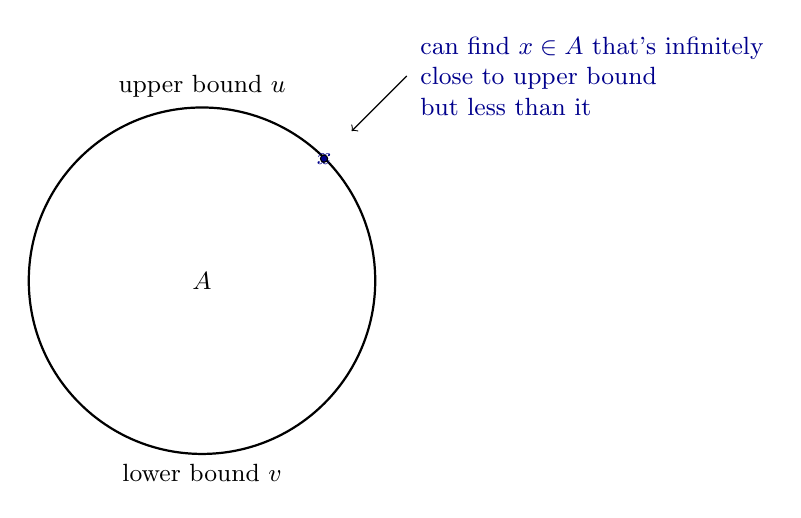
\begin{tikzpicture}[scale=1, every node/.style={font=\small}]
    \draw[thick] (0,0) circle (2.2cm);
    \node at (0,0) {$A$};
    \node[blue!55!black] at (1.55,1.55) {$x$};
    \draw[fill=blue!55!black] (1.55,1.55) circle (1.3pt);
    \node[above] at (0,2.2) {upper bound $u$};
    \node[below] at (0,-2.2) {lower bound $v$};
    \draw[->] (2.6,2.6) -- (1.9,1.9);
    \node[align=left, blue!55!black, anchor=west] at (2.65,2.6) {\text{\shortstack[l]{can find $x \in A$ that's infinitely\\ close to upper bound\\ but less than it}}};
\end{tikzpicture}
\end{center}

\begin{example}
    \[A = (0,1)\]
    \[\sup A = 1 \qquad \inf A = 0\]
\end{example}

\heading{Distinction of sup/inf vs.\ max/min:}
$\max(A)$ and $\min(A)$ must be elements of the set $A$.
\\ $\sup(A)$ and $\inf(A)$ may not be elements of $A$.

\begin{example}
    \[A = (0,1)\]
    $\max(A)$ and $\min(A)$ do not exist. $\sup(A)$ and $\inf(A)$ do exist.
    \[B = (0,1]\]
    $\min(B)$ does not exist, $\max(B) = 1$. $\sup(B) = 1$, $\inf(B) = 0$.
\end{example}

\deflabel{1.2.3}{Limsup and Liminf}
\begin{quote}
    Let $(x_n) \subseteq \R$ be a sequence.
    \[\limsup_{n\to\infty} x_n = \lim_{n\to\infty}\ \sup_{m\geq n} x_m = \inf_{n\geq 0}\ \sup_{m\geq n} x_m\]
    \[\liminf_{n\to\infty} x_n = \lim_{n\to\infty}\ \inf_{m\geq n} x_m = \sup_{n\geq 0}\ \inf_{m\geq n} x_m\]
\end{quote}

\begin{center}
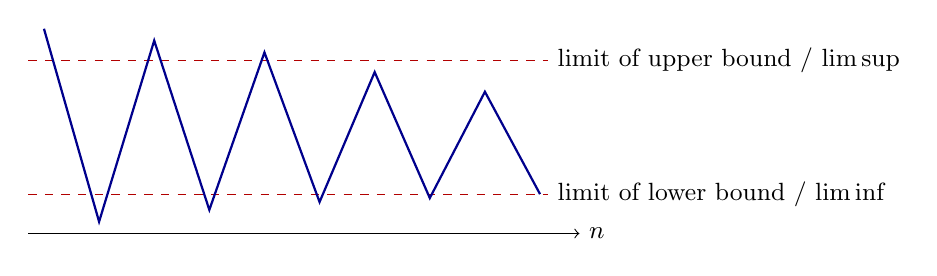
\begin{tikzpicture}[scale=1, every node/.style={font=\small}]
    \draw[->] (0,0) -- (7,0) node[right]{$n$};
    \draw[dashed, red!70!black] (0,2.2) -- (6.6,2.2) node[right, black]{\text{limit of upper bound / $\limsup$}};
    \draw[dashed, red!70!black] (0,0.5) -- (6.6,0.5) node[right, black]{\text{limit of lower bound / $\liminf$}};
    \draw[thick, blue!55!black]
        (0.2,2.6) -- (0.9,0.15) -- (1.6,2.45) -- (2.3,0.3) -- (3,2.3)
        -- (3.7,0.4) -- (4.4,2.05) -- (5.1,0.45) -- (5.8,1.8) -- (6.5,0.5);
\end{tikzpicture}
\end{center}

\begin{example}
    \[x_n = (-1)^n = -1,1,-1,1,\dots\]
    No limit, diverges: $\displaystyle\lim_{n\to\infty} x_n$ DNE.
    \\ But $\displaystyle\sup_{m\geq n} x_m = 1$ and $\displaystyle\inf_{m\geq n} x_m = -1$
    \[\Rightarrow \limsup_{n\to\infty} x_n = 1, \qquad \liminf_{n\to\infty} x_n = -1\]
\end{example}

\text{The limsup and liminf are used to describe the long-run behaviour of a sequence, even if the sequence does not converge.}
\\ For a sequence $x_n$, if $\displaystyle\limsup_{n\to\infty} x_n = \liminf_{n\to\infty} x_n = x$, then $\displaystyle\lim_{n\to\infty} x_n = x$.

\subsection{Function Limits}

\deflabel{1.3}{Left and Right Limit of a Function}
\begin{quote}
    For any function $f: \R \to \R$,
    \[f(x-) = \lim_{y\uparrow x} f(y) = L \quad \text{(to the left of $x$, a small neighbourhood)}\]
    \[\Leftrightarrow \forall \varepsilon>0,\ \exists \delta>0 \text{ s.t. } \forall y \in (x-\delta,x),\ \left\lvert f(y)-L\right\rvert < \varepsilon.\]
    \[f(x+) = \lim_{y\downarrow x} f(y) = U\]
    \[\Leftrightarrow \forall \varepsilon>0,\ \exists \delta>0 \text{ s.t. } \forall y \in (x,x+\delta),\ \left\lvert f(y)-U\right\rvert < \varepsilon.\]
    If $f(x-) = f(x+) = C$, then $\textcolor{blue!55!black}{\displaystyle\lim_{y\to x} f(y) = C}$.
\end{quote}

\begin{example}
    \[f(x) = \begin{cases} 0 & x<0 \\ 1 & x\geq 0 \end{cases}\]
    $f(0-) = 0$, $f(0+) = 1$
    \[\Rightarrow \lim_{x\to 0} f(x) \text{ DNE}\]
\end{example}

\chapterentry{Chapter 2: Probability Measure}
% !TeX root = ../main.tex

\newlecture[Probability Measure][Sep 10, 2026]

\deflabel{2.1}{Sample Space}
\begin{quote}
    A sample space $\Omega$ is any non-empty set.
\end{quote}

\begin{example}[][2.1]
    The sample space contains ``all the states of the following''
    \\Coin Flipping: $\Omega = \{H, T\}$
    \\Weather: $\{\text{hot, cold, mild}\} \times \{\text{wet, dry}\}$
\end{example}

\deflabel{2.2}{Probability Measure (STA347 ver.)}
\begin{quote}
    For a sample space $\Omega$, we say $P$ is a probability measure if the following holds:
    \begin{enumerate}[label=\roman*)]
        \item $\forall E \subseteq \Omega, 0 \leq P(E) \leq 1$, that is $P:\mathcal{P}(\Omega) \to [0,1]$
        \item $P(\Omega) = 1$
        \item $\forall E_1, E_2, \dots \subseteq \Omega$ such that $E_i \cap E_j = \varnothing \ \quad\forall\ i \neq j$
        \[P\left(\bigcup_{i=1}^{\infty} E_i\right) = \sum_{i=1}^{\infty}P(E_i)\]
    \end{enumerate}
\end{quote}

\text{$\mathcal{P}(\Omega)$ is the power set of $\Omega$.}

\textbf{Remark:} It may be impossible for such a $P$ to exist. To define exactly which subsets we want $P$ to satisfy these axioms, that would require more advanced mathematical theories. For this class, we just assume such a $P$ is defined for all subsets of $\Omega$.

\begin{example}[Probabilities of Coin Flipping][2.2]
    \[\Omega = \{H, T\}\]
    \[\mathcal{P}(\Omega) = \{\phi, \{H\}, \{T\}, \{H, T\}\}\]
    \[P: \mathcal{P}(\Omega) \mapsto [0, 1]\]
    \begin{align*}
        P: \phi &\mapsto 0 \\
        \{H\} &\mapsto \frac{1}{2} \\
        \{T\} &\mapsto \frac{1}{2} \\
        \{H, T\} &\mapsto 1
    \end{align*}
\end{example}

\begin{example}[The Uniform/Lebesgue Measure][2.3]
    Let $\Omega =[L,U]$ for some $L < U \in \R$. Define
    \[P([a,b]) = \frac{b-a}{U-L} \quad \text{when } L \leq a \leq b \leq U\]
    We assume such a measure exists (and is well defined) for this class.
\end{example}

\begin{proposition}[][2.3]
The following properties are satisfied by any probability measure $P$
\begin{enumerate}
    \item $\forall E \subseteq \Omega, P(E^C) = 1 - P(E)$
    \item $P(\phi) = 0$
    \item $\forall E, F \subseteq \Omega$, such that $E \subseteq F, P(E) \leq P(F)$ \text{(``big event, big probability'')}
    \item $\forall E, F \subseteq \Omega, P(E\bigcup F) = P(E)+P(F) - P(E\bigcap F)$
    \item $\forall E, F \subseteq \Omega, P(E\bigcap F) = P(E)+P(F)-P(E\bigcup F)$
    \item $\forall E, F \subseteq \Omega, P(F \setminus E) = P(F) - P(E\bigcap F)$
\end{enumerate}
Proof via Def 2.2 (probability axioms).
\end{proposition}

\begin{lemma}[][2.4]
    For a sequence $E_1, \dots, E_n \subseteq \Omega$
    \[P(\bigcup_{i=1}^n E_i) \leq \sum_{i=1}^{n}P(E_i)\]
    \begin{proof}
    We define $F_i = E_i \setminus \bigcup_{j=1}^{i-1}E_j, F_1 = E_1$
    \[\bigcup_{i=1}^{n} E_i = \bigcup_{i=1}^{n}F_i \text{ and } F_i \bigcap F_j = \phi \text{ if } i \neq j\]
    \begin{center}
    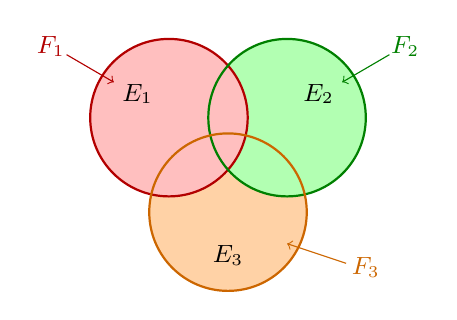
\begin{tikzpicture}[scale=1, every node/.style={font=\small}]
        % painter's order: E3 first, then E2 on top, then E1 on top,
        % so each visible colour is exactly F_i = E_i minus earlier E_j
        \fill[orange!35] (0.15,-1.2) circle (1);
        \fill[green!30] (0.9,0) circle (1);
        \fill[red!25] (-0.6,0) circle (1);
        \draw[thick, red!70!black] (-0.6,0) circle (1);
        \draw[thick, green!50!black] (0.9,0) circle (1);
        \draw[thick, orange!80!black] (0.15,-1.2) circle (1);
        \node at (-1.0,0.3) {$E_1$};
        \node at (1.3,0.3) {$E_2$};
        \node at (0.15,-1.75) {$E_3$};
        \node[red!70!black] at (-2.1,0.9) {$F_1$};
        \draw[->, red!70!black] (-1.9,0.8) -- (-1.3,0.45);
        \node[green!50!black] at (2.4,0.9) {$F_2$};
        \draw[->, green!50!black] (2.2,0.8) -- (1.6,0.45);
        \node[orange!80!black] at (1.9,-1.9) {$F_3$};
        \draw[->, orange!80!black] (1.65,-1.85) -- (0.9,-1.6);
    \end{tikzpicture}
    \\ \text{$F_i$ = the part of $E_i$ not already covered by $E_1,\dots,E_{i-1}$.}
    \end{center}
    from the probability axiom.
    \begin{align*}
        \text{Since } \bigcup_{i=1}^{n} E_i &= \bigcup_{i=1}^{n}F_i\\
        P(\bigcup_{i=1}^{n} E_i) &= P(\bigcup_{i=1}^{n}F_i)\\
        &= \sum_{i=1}^{n}P(F_i)
    \end{align*}
    \[\text{We also know } F_i \subseteq E_i \text{ as } F_i = E_i \setminus \bigcup_{j=1}^{i-1}E_j\]
    \[P(F_i) \leq P(E_i)\]
    \[P(\bigcup_{i=1}^{n}E_i) = \sum_{i=1}^{n}P(F_i) \leq \sum_{i=1}^{n}P(E_i)\]
    \end{proof}
\end{lemma}

\begin{lemma}[][2.5]
    Let $P$ be the Lebesgue measure on $[0,1]$. Then $P(E) = 0$ for any \underline{countable} set $E$.
\end{lemma}

\chapterentry{Chapter 3: Independence, Random Variables and Distributions}
% !TeX root = ../main.tex


\newlecture[Independence, Random Variables and Distributions][Sep 15, 2026]

\deflabel{2.7}{Independence}
\begin{quote}
    Events $E_1, \dots, E_n \subseteq \Omega$ are independent with respect to a probability measure $P$, if for each $\mathcal{I} \subseteq \underset{\text{any subset of} \left\{1, \dots, n\right\}}{[n]}$
    \[P\left(\bigcap_{i\in\mathcal{I}}E_i\right) = \prod_{i\in\mathcal{I}}P(E_i)\]
\end{quote}
e.g. if $\mathcal{I} = \left\{1,2,3\right\}$ a subset of $\left\{1,\dots,n\right\}$
\[P(E_1 \bigcap E_2 \bigcap E_3) = P(E_1)P(E_2)P(E_3)\]

\begin{reqproof}
\begin{proposition}[][2.7.1]\req{p2.7.1}\reqtoc{p2.7.1}{Prop 2.7.1}
    If $E_1, \dots E_n$ are independent, then $E_1^c, \dots, E_n^c$ are also independent. Proof as an exercise.
\end{proposition}
\end{reqproof}

\begin{reqnoproof}
\begin{proposition}[][2.7.2]\req{p2.7.2}
    If an infinite collection of events $\left\{E_\alpha :\alpha \in \mathcal{I}\right\}$ are independent, then for a finite subset $\mathcal{J} \subseteq \mathcal{I}$, the events $\left\{E_\beta : \beta \in \mathcal{J}\right\}$ are independent.
\end{proposition}
\end{reqnoproof}

\subsection{Random Variables and Distributions}
\begin{definition}[Random Variables][3.1]
    Given a sample space $\Omega$, a function $X: \Omega \rightarrow \mathbb{R}$ is a random variable.
\end{definition}

\begin{example}[Coin Flipping][3.1.1]
    \[\Omega = \left\{H, T\right\}\]
    \[\downarrow \text{R.V. } X: \quad X(H)\rightarrow 1, \quad X(T)\rightarrow 0 \]
    \[\mathbb{R}\]
\end{example}

\begin{theorem}[Distribution][3.2]
    A random variable $X$ and probability measure $P$ induce a probability measure $\mu$ on $\R$ defined by
    \[\mu(A) = P(X \in A) = P(\left\{\omega\in \Omega: X(\omega)\in A\right\})\]
    for any $A \subseteq \R$.
    \text{$\mu$ is a measure on the real number set: $\mu(\{0,1\})$ and $\mu([0,1))$ each return a certain value.}
    \\ $\mu(A)$ takes a real number set $A$ as input, and equals $P$ of the \text{pre-image of $A$ w.r.t.\ r.v.\ $X$}, i.e.\ $P(\Omega_A) = \mu(A)$ where $\Omega_A = \left\{\omega\in\Omega: X(\omega)\in A\right\}$.
\end{theorem}

\begin{example}[][3.2.1]
    Define the following
    \[\Omega = \left\{ \text{\textcolor{blue}{blue}, \textcolor{red}{red}, \textcolor{green}{green}, \textcolor{yellow}{yellow}} \right\} \]
    \[X: \begin{cases}
        \textcolor{blue}{\text{blue} \rightarrow 1} \\
        \textcolor{red}{\text{red} \rightarrow 3} \\
        \textcolor{green}{\text{green} \rightarrow 4} \\
        \textcolor{yellow}{\text{yellow} \rightarrow 6}
    \end{cases}\]

    \[P: \{\text{blue}\}\mapsto\tfrac{1}{5},\quad \{\text{red}\}\mapsto\tfrac{1}{5},\quad \{\text{green}\}\mapsto\tfrac{1}{4},\quad \{\text{yellow}\}\mapsto 1-\tfrac{1}{5}-\tfrac{1}{5}-\tfrac{1}{4}=\tfrac{7}{20}\]
    \[P(\{\text{blue, red}\}) = \tfrac{1}{5}+\tfrac{1}{5} = \tfrac{2}{5}\]
    \[A = [1,3] \]
    \begin{center}
    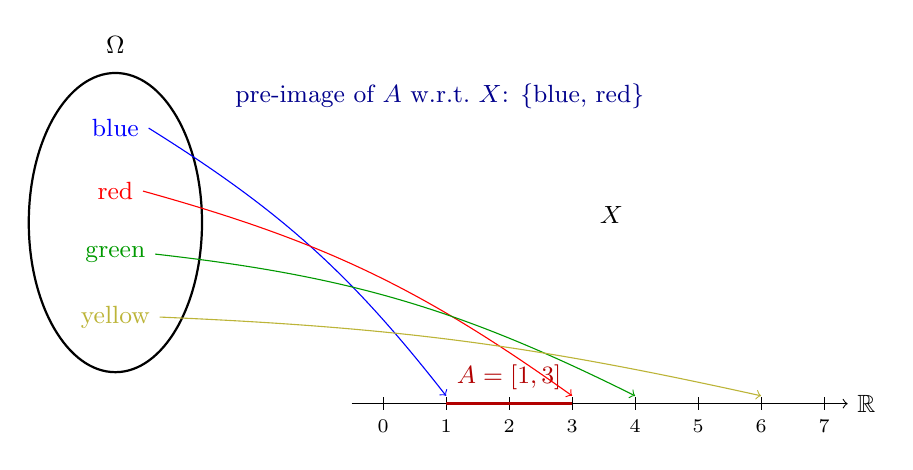
\begin{tikzpicture}[scale=1, every node/.style={font=\small}]
        \draw[thick] (0,0) ellipse (1.1cm and 1.9cm);
        \node at (0,2.25) {$\Omega$};
        \foreach \y/\col/\nm in {1.2/blue/blue, 0.4/red/red, -0.4/green!60!black/green, -1.2/yellow!70!black/yellow}
            \node[\col] (w\nm) at (0,\y) {\nm};
        \draw[->] (3,-2.3) -- (9.3,-2.3) node[right]{$\R$};
        \foreach \x in {0,...,7} \draw (3.4+0.8*\x,-2.22) -- (3.4+0.8*\x,-2.38) node[below]{\scriptsize $\x$};
        \draw[very thick, red!70!black] (4.2,-2.3) -- (5.8,-2.3);
        \node[red!70!black, above] at (5,-2.25) {$A=[1,3]$};
        \draw[->, blue] (wblue.east) to[bend left=10] (4.2,-2.2);
        \draw[->, red] (wred.east) to[bend left=10] (5.8,-2.2);
        \draw[->, green!60!black] (wgreen.east) to[bend left=10] (6.6,-2.2);
        \draw[->, yellow!70!black] (wyellow.east) to[bend left=5] (8.2,-2.2);
        \node[blue!55!black, align=left, anchor=west] at (1.4,1.6) {\text{pre-image of $A$ w.r.t.\ $X$: $\{\text{blue, red}\}$}};
        \node at (6.3,0.1) {$X$};
    \end{tikzpicture}
    \end{center}
    \begin{enumerate}
        \item $\left\{w: w \in \Omega, X(w) \in A \right\} = \left\{\text{\textcolor{blue}{blue} ,\textcolor{red}{red}}\right\}$
        \item $P(\left\{\text{\textcolor{blue}{blue} ,\textcolor{red}{red}}\right\}) = \frac{2}{5}$, so $\mu(A) = \frac{2}{5}$
    \end{enumerate}
    in summary
    \[\mu([1,3]) = \frac{2}{5}\]
\end{example}

\textbf{Claim:} $\mu$ is a probability measure on $\mathbb{R}$ (for any real number set $B$).
\begin{proof}
\begin{enumerate}
    \item $\mu(B) \in [0,1]$ is trivial, since $P$ is a probability measure.
    \item Since $X(\omega) \in \R$ for all $\omega \in \Omega$.
    \[\mu(\R) = P(\underset{\Omega}{ \left\{\omega : \omega \in \Omega, X(\omega)\in \R\right\} }) = P(\Omega) = 1\]
    \item Consider disjoint sets $A_1, A_2, \dots \subseteq \R$ and define $E_i = \left\{\omega: X(\omega) \in A_i\right\}$
    \\(e.g. $E_1 = \left\{\omega: X(\omega)\in A_1\right\}$, $E_2 = \left\{\omega: X(\omega)\in A_2\right\}$)
    \\Since $X$ is a function, it is impossible for $X(\omega) = a$ and $X(\omega) = b$ when $a\neq b$, so the $E_i$'s are also disjoint. Then
    \begin{align*}
        \mu\left(\bigcup_{i=1}^{\infty}A_i\right) &= P\left(X(\omega) \in \bigcup_{i=1}^{\infty}A_i\right) \\
        &= P\left(\bigcup_{i=1}^{\infty}E_i\right) \quad \text{we know } E_i\text{'s are disjoint} \\
        &= \sum_{i=1}^{\infty}P(E_i) \\
        &= \sum_{i=1}^{\infty}\mu(A_i)
    \end{align*}
\end{enumerate}
\end{proof}

\begin{definition}[The Cumulative Distribution Function][3.3]
    A random variable $X$ and measure $P$ generate the cumulative distribution function (CDF) defined by
    \[F(x) = \mu((-\infty, x]) = P(X \leq x)\]
    where $P(X\leq x)$ is a short-hand notation for
    \[P(\left\{\omega: \omega \in \Omega, X(\omega) \in (-\infty, x]\right\})\]
\end{definition}

\begin{theorem}[][3.3.1]
    A distribution function $F$ for a random variable $X$ uniquely defines the measure $\mu$.
    \\Proof is outside the scope of this class.
\end{theorem}

\begin{example}[Uniform Distribution][3.3.2]
    $P$ is uniform on $[0,1]$ and $X(\omega)=\omega$
    \\For $x\in[0,1)$
    \begin{align*}
        F(x) &= \mu((-\infty, x]) & \leftarrow& \text{by definition of CDF} \\
        &= P(X \leq x) & \leftarrow& \text{by Thm 3.2 (definition of distribution)} \\
        &= P\left(\left\{\omega :X(\omega) \in (-\infty, x]\right\}\right) \\
        &= P((-\infty, x]) & \leftarrow& \text{by }X(\omega) = \omega \\
        &= P([0,x]) & \leftarrow& \text{because $P$ is a uniform/Lebesgue measure} \\
        &= x
    \end{align*}
\end{example}

\begin{theorem}[Properties of Distribution Function][3.4]
    A distribution function satisfies the following properties:
    \begin{enumerate}[label = \roman*)]
        \item For all $x \leq y \in \R, F(x) \leq F(y)$
        \item $\lim_{x \to -\infty} F(x) = 0 $ and $\lim_{x \to +\infty} F(x) = 1 $
        \item $F$ is right-continuous
    \end{enumerate}
    \begin{proof}
        \begin{enumerate}[label = \roman*)]
            \item $x\leq y \in \R$
            \[F(x) = \mu((-\infty, x]), F(y) = \mu((-\infty, y])\]
            Since $x\leq y$, \quad $(-\infty, x] \subseteq (-\infty, y]$
            \[\mu((-\infty, x])\leq \mu((-\infty, y])\]
            ``bigger set, bigger probability''
            \[(A \subseteq B, \quad P(A) \leq P(B) \quad / \quad \mu(A)\leq \mu(B))\]
            \item Define $A_n = \left\{X\leq -n\right\}, \quad n\geq 0$
            \\Then $A_1 \supseteq A_2 \supseteq A_3 \supseteq \dots $
            \begin{center}
            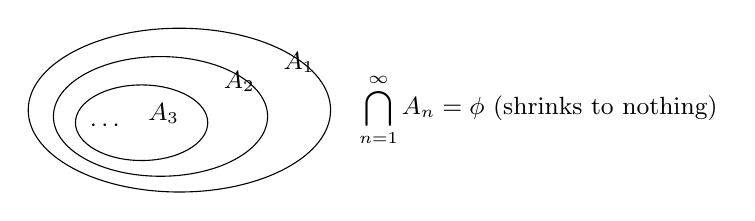
\begin{tikzpicture}[scale=0.8, every node/.style={font=\small}]
                \draw (0,0) ellipse (2.4cm and 1.3cm);
                \draw (-0.3,-0.1) ellipse (1.7cm and 0.95cm);
                \draw (-0.6,-0.2) ellipse (1.05cm and 0.6cm);
                \node at (1.9,0.75) {$A_1$};
                \node at (0.95,0.45) {$A_2$};
                \node at (-0.25,-0.05) {$A_3$};
                \node at (-1.15,-0.25) {$\cdots$};
                \node[anchor=west] at (2.7,0) {$\displaystyle\bigcap_{n=1}^{\infty} A_n = \phi$ \text{(shrinks to nothing)}};
            \end{tikzpicture}
            \end{center}
            \begin{align*}
                \bigcap_{n=1}^{\infty} A_n &= \phi \\
                \lim_{n \to \infty} F(-n) &= \lim_{n \to \infty} P(A_n) \\
                &= P\left(\bigcap_{n=1}^{\infty}A_n\right) \\
                &= P(\phi) = 0
            \end{align*}
            Define $B_n = \left\{X\leq n\right\}$,
            \\then $B_1 \subseteq B_2 \subseteq \dots$
            \begin{center}
            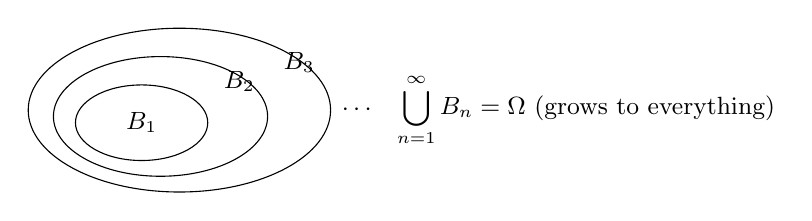
\begin{tikzpicture}[scale=0.8, every node/.style={font=\small}]
                \draw (-0.6,-0.2) ellipse (1.05cm and 0.6cm);
                \draw (-0.3,-0.1) ellipse (1.7cm and 0.95cm);
                \draw (0,0) ellipse (2.4cm and 1.3cm);
                \node at (-0.6,-0.2) {$B_1$};
                \node at (0.95,0.45) {$B_2$};
                \node at (1.9,0.75) {$B_3$};
                \node at (2.85,0) {$\cdots$};
                \node[anchor=west] at (3.3,0) {$\displaystyle\bigcup_{n=1}^{\infty} B_n = \Omega$ \text{(grows to everything)}};
            \end{tikzpicture}
            \end{center}
            \[\bigcup_{n=1}^{\infty} B_n = \Omega\]
            \begin{align*}
                \lim_{n \to \infty} F(n) &= \lim_{n \to \infty} P(B_n) \\
                &= P\left(\bigcup_{n=1}^{\infty}B_n\right) \\
                &= P(\Omega) = 1
            \end{align*}
            \item Fix $x\in \R$ and let $h_n \downarrow 0 \quad (h_n \geq 0 \quad h_n \rightarrow 0, h_1 \geq h_2 \geq \dots)$
            \\Define $C_n = \left\{X\leq x+h_n\right\}$
            \\then $C_1 \supseteq C_2 \supseteq \dots$
            \[\lim_{n \to \infty} C_n = \bigcap_{n=1}^{\infty} C_n = \left\{X\leq x\right\} \]
            Therefore
            \[\lim_{n \to \infty} F(x+h_n) = \lim_{n \to \infty} P(C_n) = P(\bigcap_{n=1}^{\infty} C_n) = P(X \leq x) = F(x) \]
            Hence
            \[\lim_{h \downarrow 0}F(x+h) = F(x)  \]
            So $F$ is right-continuous.
        \end{enumerate}
    \end{proof}
\end{theorem}

\begin{definition}[The Inverse CDF][3.5]
    The inverse CDF of a r.v. $X$ is defined by
    \[F^{-1}(y) = \sup\left\{x:F(x) < y\right\}\]
\end{definition}

\begin{reqnoproof}
\begin{theorem}[][3.5.1]\req{t3.5.1}
    If $F$ satisfies properties i) to iii) of Thm 3.4, then such an $F$ is the CDF of some r.v. 
\end{theorem}
\end{reqnoproof}

\begin{theorem}[][3.6]
    If $F$ is a CDF, it can only have countably many discontinuities.
\end{theorem}

% !TeX root = ../main.tex

\newlecture[Random Variables \& Distributions][Sep 17, 2026]
\begin{definition}[Density Function][3.7]
    A random variable has a density function
    \[f: \mathbb{R} \rightarrow \mathbb{R}, \quad \text{if for all }x \in \mathbb{R} \]
    \[F(x) = \int_{-\infty}^{x}f(y)\,dy\]
    we call $f(\cdot)$ the density function.
\end{definition}

\begin{definition}[Joint Distribution][3.8]
    We define the joint distribution function of a random vector $\overrightarrow{X} = (X_1, \dots, X_n)$ by
    \[F(x_1, \dots, x_n) = P(X_1 \leq x_1, \dots, X_n \leq x_n)\]
    using the notation $P(A, B) \overset{def}{=}P(A\bigcap B)$
\end{definition}

\begin{theorem}[][3.8.1]
    A joint distribution function $F: \mathbb{R}^n \rightarrow \mathbb{R} $ satisfies the following properties:
    \begin{enumerate}[label = \roman*)]
        \item if $(x_1, \dots, x_n)$ and $(x_1', \dots, x_n')$ satisfy $x_i \leq x_i'$ for all $i \in [n]$,
        \[F(x_1, \dots x_n) \leq F(x_1', \dots x_n')\]
        \item $\lim_{x_i \to -\infty} F(x_1, \dots, x_n) = 0$ for all $i \in \left\{1, \dots, n\right\}$ and 
        $\lim_{x_1 \to \infty, \dots x_n \to \infty}  F (x_1, \dots, x_n) = 1$
        \item $\lim_{h \to 0^+}F(x_1+h, \dots, x_n) = \cdots = \lim_{h \to 0^+}F(x_1, \dots x_n+h)$
        \[=F(x_1, \dots, x_n)\]
    \end{enumerate}
    Proofs are analogous to the proofs under the univariate case.
\end{theorem}

\begin{reqnoproof}
\begin{definition}[The Joint Density][3.9]\req{d3.9}
    A random vector has a joint density function:
    \[f: \mathbb{R}^n \to \mathbb{R}, \quad \text{if }\forall(x_1, \dots, x_n)\in \mathbb{R}^n\]
    \[F(x_1, \dots x_n) = \int_{-\infty}^{x_1}\cdots \int_{-\infty}^{x_n}f(y_1, \dots, y_n)\, dy_n\dots \,dy_1\]
\end{definition}
\end{reqnoproof}

\begin{reqnoproof}
\begin{theorem}[Independence of Random Variables][3.10]\req{t3.10}
    Random variables $X_1, \dots, X_n$ with CDFs $F_1, \dots, F_n$
    are independent if and only if
    \[F(x_1, \dots, x_n) = \prod_{i=1}^nF_i(x_i), \quad \forall(x_1, \dots, x_n) \in \mathbb{R}^n \]
\end{theorem}
\end{reqnoproof}

\heading{Limits of sets:}
Let $A_i$ be sets for $i\in\{1,2,\dots\}$ and consider $\displaystyle\lim_{n\to\infty}A_n$.
\begin{itemize}
    \item If $A_1 \subseteq A_2 \subseteq \dots \subseteq A_n \subseteq \dots$ (increasing), then $\displaystyle\lim_{n\to\infty}\bigcup_{i=1}^{n}A_i = \bigcup_{i=1}^{\infty}A_i$.
    \item If $A_1 \supseteq A_2 \supseteq \dots \supseteq A_n \supseteq \dots$ (decreasing), then $\displaystyle\lim_{n\to\infty}\bigcap_{i=1}^{n}A_i = \bigcap_{i=1}^{\infty}A_i$.
\end{itemize}
\begin{center}
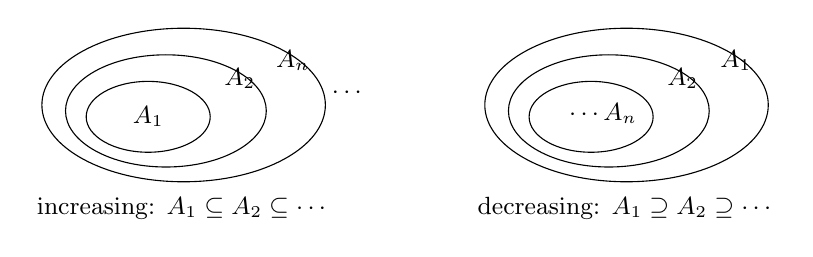
\begin{tikzpicture}[scale=0.75, every node/.style={font=\small}]
    % increasing
    \draw (-0.6,-0.2) ellipse (1.05cm and 0.6cm);
    \draw (-0.3,-0.1) ellipse (1.7cm and 0.95cm);
    \draw (0,0) ellipse (2.4cm and 1.3cm);
    \node at (-0.6,-0.2) {$A_1$};
    \node at (0.95,0.45) {$A_2$};
    \node at (1.85,0.75) {$A_n$};
    \node at (2.8,0.2) {$\cdots$};
    \node at (0,-1.75) {\text{increasing: $A_1 \subseteq A_2 \subseteq \cdots$}};
    % decreasing
    \begin{scope}[xshift=7.5cm]
        \draw (0,0) ellipse (2.4cm and 1.3cm);
        \draw (-0.3,-0.1) ellipse (1.7cm and 0.95cm);
        \draw (-0.6,-0.2) ellipse (1.05cm and 0.6cm);
        \node at (1.85,0.75) {$A_1$};
        \node at (0.95,0.45) {$A_2$};
        \node at (-0.4,-0.15) {$\cdots A_n$};
        \node at (0,-1.75) {\text{decreasing: $A_1 \supseteq A_2 \supseteq \cdots$}};
    \end{scope}
\end{tikzpicture}
\end{center}

\chapterentry{Expectation}
% !TeX root = ../main.tex

\newlecture[Expectation][Sep 22, 2026]
\subsection{Expectation}

In STA237:
\[E(X) = \begin{cases*}
    \sum_{x}^{}x\cdot p(x) &\text{if } X \text{ discrete}\\
    \int xf(x)\,dx &\text{if } X \text{ continuous}
\end{cases*}\]
for this course, we are defining probability via ``measure theory'', so we need to revisit the definition of expectation.

Particularly, under the ``measure theory'' perspective:
\[E(X) = \int x\, dP \quad \Rightarrow P = \text{probability measure}\]
\[\int xf(x)\,dx \quad \Rightarrow \quad \int x\, dP\]
``Riemann Integral''

\begin{definition}[Simple Expectation][5.1]
    If $X$ only takes finitely many values $x_1, \dots, x_n$, and $A_i = \left\{\omega: X(\omega) = x_i\right\}$, define the expectation of $X$ by:
    \[E(X) = \sum_{i=1}^{n}x_i P(A_i)\]
\end{definition}

\begin{example}[][5.1.1]
    For an arbitrary set $A \subset \Omega$, let
    \[Y(\omega) = I\left\{\omega \in A\right\} \qquad \text{Then } E(Y) = P(A)\]
    \begin{align*}
        E(Y) &= \sum_{i=0}^{1}y_i \cdot P(A_i) \qquad Y\text{ only takes two values 0 and 1}\\
        &= 1 \cdot P\left\{\omega \in A\right\} + 0\cdot P\left\{\omega \notin A\right\}\\
        &= P(A) = P(\left\{\omega: \omega \in A\right\})
    \end{align*}
\end{example}


\begin{example}[][5.1.2]
    $P$ is uniform measure on $\Omega = [0,1)$, and
    \[X(\omega) = \begin{cases}
        5 & \omega > \frac{1}{3} \\
        3 & \omega \leq \frac{1}{3}
    \end{cases}\]
    \begin{center}
    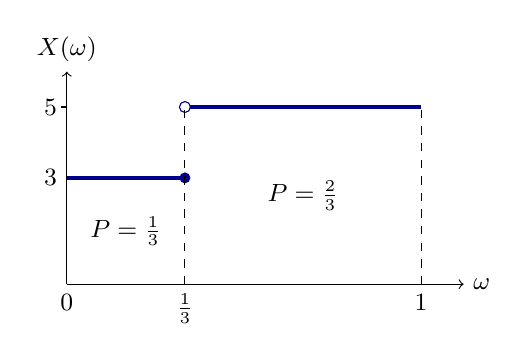
\begin{tikzpicture}[xscale=4.5, yscale=0.45, every node/.style={font=\small}]
        \draw[->] (0,0) -- (1.12,0) node[right]{$\omega$};
        \draw[->] (0,0) -- (0,6) node[above]{$X(\omega)$};
        \draw[very thick, blue!55!black] (0,3) -- (1/3,3);
        \draw[very thick, blue!55!black] (1/3,5) -- (1,5);
        \node[circle, fill=blue!55!black, inner sep=1.4pt] at (1/3,3) {};
        \node[circle, draw=blue!55!black, fill=white, inner sep=1.4pt] at (1/3,5) {};
        \draw[dashed] (1/3,0) -- (1/3,5);
        \draw[dashed] (1,0) -- (1,5);
        \node[below] at (0,0) {$0$};
        \node[below] at (1/3,0) {$\frac{1}{3}$};
        \node[below] at (1,0) {$1$};
        \node[left] at (0,3) {$3$};
        \node[left] at (0,5) {$5$};
        \draw (0,5) -- (-0.015,5);
        \node at (1/6,1.5) {\text{$P = \frac13$}};
        \node at (2/3,2.5) {\text{$P = \frac23$}};
    \end{tikzpicture}
    \end{center}
    \[E(X) = 5 \cdot P(\omega > \frac{1}{3}) + 3\cdot P(\omega \leq \frac{1}{3})\]
    \[=5\cdot (1-\frac{1}{3}) + 3\cdot \frac{1}{3}\]
    \[ = \frac{13}{3}\]
\end{example}

\begin{proposition}[Properties of Expectation][5.2]
    If $X$ and $Y$ are simple random variables, the following hold:
    \begin{enumerate}[label = \roman*)]
        \item If $X\geq 0$ a.s., $E(X) \geq 0$
        \item For any $a \in \mathbb{R}$, $E(aX) = a \cdot E(X)$
        \item $E(X+Y) = E(X)+E(Y)$
    \end{enumerate}
    Remark: "a.s." means almost surely.
    if $E$ a.s. $\Rightarrow$ $P(E) = 1$
    \\  $X \geq 0$ a.s. $\Rightarrow$ $P(X \geq 0) = 1$ $\Leftrightarrow$ $P(\left\{\omega: X(\omega) \geq 0\right\})=1$
    \\we may have certain $\omega$'s s.t. $X(\omega) < 0$, but $P(\left\{\omega: X(\omega) < 0\right\}) = 0$
\end{proposition}

\begin{proof}
Both i) and ii) are trivial.
\\For iii), let $X$ take values $x_1, \dots, x_n$ on sets $A_1,\dots, A_n$ (i.e. $A_i = \left\{\omega: X(\omega) = x_i\right\}$) and $Y$ takes values $y_1, \dots, y_m$ on sets $B_1, \dots, B_m$.
\\Observe that there are $m\cdot n$ events
\[C_{ij} = \left\{X = x_i \bigcap Y = y_j \right\}\]
Then
\begin{align*}
    E(X+Y) &= \sum_{i=1}^{n}\sum_{j=1}^{m} (x_i+y_j)\cdot P(C_{ij})\\
    &= \sum_{i=1}^{n}x_i \sum_{j=1}^{m} P(X=x_i \cap Y=y_j)+\sum_{j=1}^{m}y_j \sum_{i=1}^{n} P(X=x_i \cap Y=y_j)\\
    &= \sum_{i=1}^{n}x_i P(X=x_i)+\sum_{j=1}^{m}y_j P(Y=y_j)\\
    &= E(X)+E(Y)
\end{align*}
\end{proof}

\begin{lemma}[][5.2.1]
    If Proposition 5.2 holds, the following properties also hold:
    \begin{enumerate}[label = \roman*), start=4]
        \item If $X \leq Y$ a.s., then $E(X) \leq E(Y)$
        \item If $X=Y$ a.s., then $E(X) = E(Y)$
        \item $\left|E(X)\right| \leq E(\left|X\right|)$
    \end{enumerate}
    proof as exercise.
\end{lemma}

Our logic is, we first define
\begin{center}
    expectation of simple random variables
    \\$\Downarrow$
    \\expectation of bounded R.V.'s (approximation)
    \\$\Downarrow$
    \\expectation of non-negative R.V's (truncation)
    \\$\Downarrow$
    \\expectation of any R.V.'s (symmetric)
\end{center}

\begin{definition}[Bounded Random Variable][5.3]
    A random variable $X$ is bounded if there exists
    $M< \infty$, such that $|X|\leq M$ a.s.
\end{definition}

\begin{definition}[Expectation of Bounded Random Variable][5.3.1]
    If $X$ is a bounded R.V., then
    \begin{align*}
        E(X) &= \inf\left\{ E(Z): Z \text{ simple, }Z \geq X \text{ a.s.}\right\}\\
        &= \sup\left\{E(Y): Y \text{ simple, }Y \leq X \text{ a.s.}\right\}
    \end{align*}
\end{definition}

Recall, when we defined the integral:
\\the integral is defined as the limit value of sums of areas of tiny rectangles.
\begin{center}
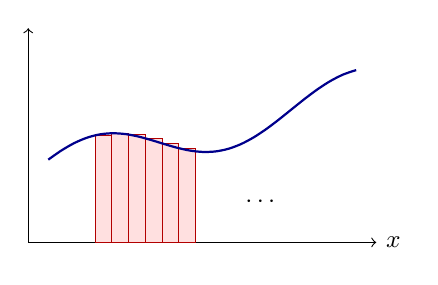
\begin{tikzpicture}[scale=0.85, every node/.style={font=\small}]
    \draw[->] (0,0) -- (5.2,0) node[right]{$x$};
    \draw[->] (0,0) -- (0,3.2);
    \foreach \x in {1.0,1.25,...,2.25} {
        \pgfmathsetmacro{\h}{0.35*sin(deg(1.6*\x))+0.25*\x+1.0}
        \draw[red!70!black, fill=red!12] (\x,0) rectangle (\x+0.25,\h);
    }
    \draw[thick, blue!55!black, domain=0.3:4.9, smooth, variable=\x] plot ({\x}, {0.35*sin(deg(1.6*\x))+0.25*\x+1.0});
    \node at (3.5,0.6) {$\cdots$};
\end{tikzpicture}
\end{center}
When it comes to the Riemann integral, we are no longer cutting $X$ axis into tiny intervals, but cutting each set into tiny subsets and calculate the sum of $x$ times the measure of each tiny subset.
\begin{align*}
    E(X) &= \inf \left\{E(Z): \quad Z\text{ is simple and } Z \geq X \text{ a.s.}\right\}\\
    &= \sup \left\{E(Y): \quad Y \text{ is simple and } Y \leq X \text{ a.s.}\right\}
\end{align*}
\begin{center}
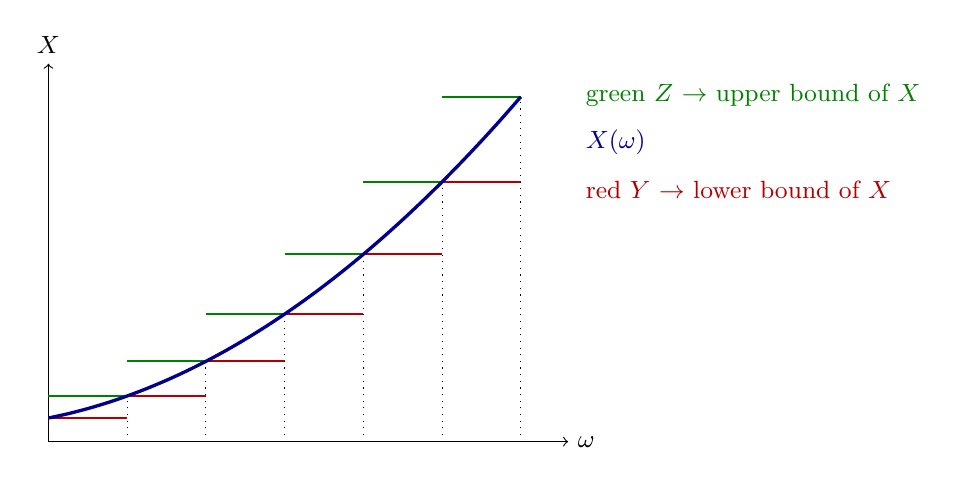
\begin{tikzpicture}[scale=1, every node/.style={font=\small}]
    \draw[->] (0,0) -- (6.6,0) node[right]{$\omega$};
    \draw[->] (0,0) -- (0,4.8) node[above]{$X$};
    \foreach \a in {0,1,...,5} {
        \pgfmathsetmacro{\lo}{0.08*\a*\a+0.2*\a+0.3}
        \pgfmathsetmacro{\hi}{0.08*(\a+1)*(\a+1)+0.2*(\a+1)+0.3}
        \draw[thick, green!50!black] (\a,\hi) -- (\a+1,\hi);
        \draw[thick, red!70!black] (\a,\lo) -- (\a+1,\lo);
        \draw[dotted] (\a+1,0) -- (\a+1,\hi);
    }
    \draw[very thick, blue!55!black, domain=0:6, smooth, variable=\x] plot ({\x}, {0.08*\x*\x+0.2*\x+0.3});
    \node[anchor=west, green!50!black] at (6.7,4.4) {green $Z$ $\to$ upper bound of $X$};
    \node[anchor=west, blue!55!black] at (6.7,3.8) {$X(\omega)$};
    \node[anchor=west, red!70!black] at (6.7,3.2) {red $Y$ $\to$ lower bound of $X$};
\end{tikzpicture}
\end{center}
``Squeeze the R.V. $X$ via two simple R.V.'s $Y$ and $Z$, with one capturing the upper bound and the other capturing the lower bound''.
\begin{proof}
Since $X$ is bounded, $|X| < M$ a.s.
\[L = \sup \left\{EY: \quad Y \text{ simple and }Y\leq X \text{ a.s.}\right\}\]
\[U = \inf\left\{EZ: \quad Z \text{ simple and }Z \geq X \text{ a.s.}\right\}\]
\[L \leq U \text{ as } Y\leq X \text{ a.s. and }Z\geq X \text{ a.s.}\]
Our goal is to prove $L \geq U \quad \Rightarrow \quad L = U \overset{def}{=}E(X)$
\\the way to cut $[-M, M]$ into tiny intervals.
\\for any arbitrary $n$, we define
\[E_k = \left\{\omega: \frac{kM}{n}\geq X(\omega) \geq \frac{(k-1)M}{n}\right\}\]
\begin{center}
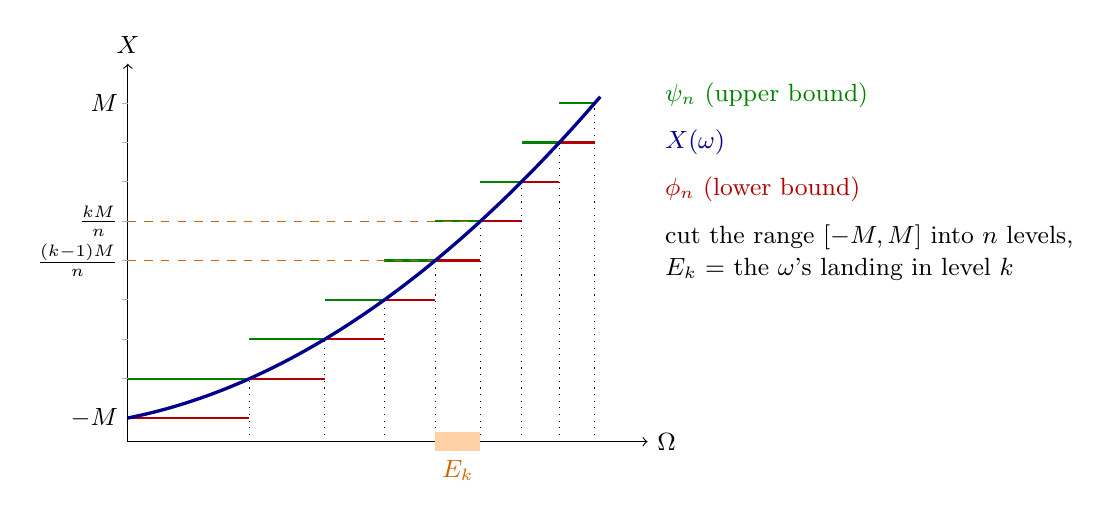
\begin{tikzpicture}[scale=1, every node/.style={font=\small}]
    % inverse of X(w) = 0.08 w^2 + 0.2 w + 0.3, to find where each level is hit
    \def\Xinv#1{(-0.2+sqrt(0.04+0.32*((#1)-0.3)))/0.16}
    \draw[->] (0,0) -- (6.6,0) node[right]{$\Omega$};
    \draw[->] (0,0) -- (0,4.8) node[above]{$X$};
    \foreach \k in {1,...,8} {
        \pgfmathsetmacro{\ylo}{0.5*\k-0.5+0.3}
        \pgfmathsetmacro{\yhi}{0.5*\k+0.3}
        \pgfmathsetmacro{\wlo}{max(0,\Xinv{\ylo})}
        \pgfmathsetmacro{\whi}{\Xinv{\yhi}}
        \draw[thick, green!50!black] (\wlo,\yhi) -- (\whi,\yhi);
        \draw[thick, red!70!black] (\wlo,\ylo) -- (\whi,\ylo);
        \draw[dotted] (\whi,0) -- (\whi,\yhi);
        \draw[gray!60] (-0.08,\yhi) -- (0,\yhi);
    }
    % highlight one E_k
    \pgfmathsetmacro{\wa}{\Xinv{2.3}}
    \pgfmathsetmacro{\wb}{\Xinv{2.8}}
    \fill[orange!35] (\wa,-0.12) rectangle (\wb,0.12);
    \node[below, orange!80!black] at ({(\wa+\wb)/2},-0.12) {$E_k$};
    \draw[dashed, orange!80!black] (0,2.3) -- (\wa,2.3);
    \draw[dashed, orange!80!black] (0,2.8) -- (\wb,2.8);
    \node[left] at (0,2.3) {$\frac{(k-1)M}{n}$};
    \node[left] at (0,2.8) {$\frac{kM}{n}$};
    \node[left] at (0,0.3) {$-M$};
    \node[left] at (0,4.3) {$M$};
    \draw[very thick, blue!55!black, domain=0:6, smooth, variable=\x] plot ({\x}, {0.08*\x*\x+0.2*\x+0.3});
    \node[anchor=west, green!50!black] at (6.7,4.4) {$\psi_n$ (upper bound)};
    \node[anchor=west, blue!55!black] at (6.7,3.8) {$X(\omega)$};
    \node[anchor=west, red!70!black] at (6.7,3.2) {$\phi_n$ (lower bound)};
    \node[anchor=west] at (6.7,2.4) {\text{\shortstack[l]{cut the range $[-M,M]$ into $n$ levels,\\ $E_k$ = the $\omega$'s landing in level $k$}}};
\end{tikzpicture}
\end{center}

we then define two simple R.V.'s
\\Lower bound: \[\phi_n(\omega) = \sum_{k}^{}\frac{(k-1)M}{n}\cdot I(\omega \in E_k)\]
\\Upper bound: \[\psi_n(\omega) = \sum_{k}^{}\frac{kM}{n}\cdot I(\omega \in E_k) \]
\[\phi_n(\omega) \leq X(\omega) \leq \psi_n(\omega)\]
\[E\phi_n(\omega) \leq E(X) \leq E\psi_n(\omega)\]
\[E\psi_n(\omega) = E\phi_n(\omega) + \frac{M}{n}\]
Let $n\to\infty$, \quad $\dfrac{M}{n} \to 0$, so the upper bound and lower bound converge:
\[L \geq E\phi_n = E\psi_n - \frac{M}{n} \geq U - \frac{M}{n} \quad \Rightarrow \quad L \geq U\]
\[E(X) = E\psi_n(\omega) = E\phi_n(\omega) \quad \text{as } n\to\infty\]
\end{proof}

$X \leq Y$ a.s. means:
\begin{enumerate}[label = step \arabic*.]
    \item $\omega: X(\omega) \leq Y(\omega)$
    \item $\left\{ \omega: X(\omega) \leq Y(\omega)\right\}$
    \item $P(\left\{ \omega: X(\omega) \leq Y(\omega)\right\}) = 1$
\end{enumerate}
then we say $X \leq Y$ a.s.

\begin{definition}[Non-negative Random Variable][5.4]
    If $X \geq 0$ a.s. ($P(\left\{\omega: X(\omega)\geq 0\right\}) = 1$)
    \\define $E(X) = \sup \left\{E(Y): Y\text{ bounded, } 0\leq Y \leq X \text{ a.s.}\right\}$
\end{definition}

\begin{center}
\begin{tikzpicture}[scale=1, every node/.style={font=\small}]
    \draw[->] (0,0) -- (6,0) node[right]{$\Omega$};
    \draw[->] (0,0) -- (0,4.5) node[above]{$X$};
    \draw[very thick, blue!55!black, domain=0.8:5.1, smooth, variable=\x] plot ({\x}, {0.6+0.5*sin(deg(\x-0.8))+0.012*(\x)^4});
    \draw[thick, red!70!black, domain=0.8:4.75, smooth, variable=\x] plot ({\x}, {min(3.2, 0.45+0.5*sin(deg(\x-0.8))+0.012*(\x)^4)});
    \draw[thick, red!70!black] (4.75,3.2) -- (5.1,3.2);
    \draw[dashed, red!70!black] (0,3.2) -- (4.75,3.2);
    \node[left, red!70!black] at (0,3.2) {bound};
    \node[anchor=west, blue!55!black] at (6.3,3.6) {$X$};
    \node[anchor=west, red!70!black] at (6.3,3.0) {$Y$: bounded, $0 \leq Y \leq X$ a.s.};
    \node[anchor=west, red!70!black] at (6.3,2.2) {$\sup\{E(Y)\} \to E(X)$};
\end{tikzpicture}
\end{center}

Remark: Def 5.4. only provides a definition of $E(X)$ when $X$ is non-negative, it does \underline{not} guarantee $E(X) < \infty$.

\begin{definition}[Integrable Random Variables][5.5]
    For any random variable $X$, let $X^+(\omega) = \max\left\{X(\omega), 0\right\}$, and $X^-(\omega) = \max\left\{-X(\omega), 0\right\}$.
    \\Observe that both $X^+$ and $X^-$ are non-negative and $X=X^+ - X^-$.
    \\Then, if $E(|X|) = E(X^+) + E(X^-) < \infty$, we say R.V. $X$ is integrable and define $E(X) = E(X^+) - E(X^-)$
\end{definition}

\begin{center}
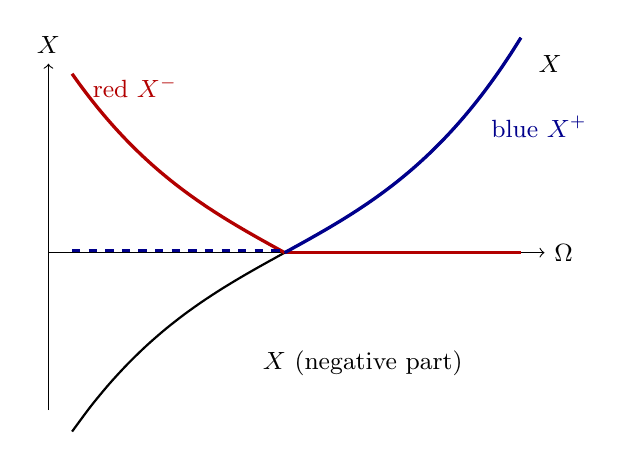
\begin{tikzpicture}[scale=1, every node/.style={font=\small}]
    \draw[->] (0,0) -- (6.3,0) node[right]{$\Omega$};
    \draw[->] (0,-2) -- (0,2.4) node[above]{$X$};
    \draw[thick, black, domain=0.3:6, smooth, variable=\x] plot ({\x}, {0.55*(\x-3)+0.04*(\x-3)*(\x-3)*(\x-3)});
    \draw[very thick, red!70!black, domain=0.3:3, smooth, variable=\x] plot ({\x}, {-0.55*(\x-3)-0.04*(\x-3)*(\x-3)*(\x-3)});
    \draw[very thick, red!70!black] (3,0) -- (6,0);
    \draw[very thick, blue!55!black, domain=3:6, smooth, variable=\x] plot ({\x}, {0.55*(\x-3)+0.04*(\x-3)*(\x-3)*(\x-3)});
    \draw[very thick, blue!55!black, dashed] (0.3,0.03) -- (3,0.03);
    \node[anchor=west] at (6.1,2.4) {$X$};
    \node[blue!55!black, anchor=west] at (5.5,1.6) {blue $X^+$};
    \node[red!70!black] at (1.1,2.1) {red $X^-$};
    \node[anchor=west] at (2.6,-1.4) {$X$ (negative part)};
\end{tikzpicture}
\end{center}

\begin{enumerate}
    \item $E|X| = E(X^+)+E(X^-) < \infty \Rightarrow X \text{ is integrable}$
    \item $E(X) = E(X^+) - E(X^-)$
\end{enumerate}

\begin{proposition}[Properties of Expected Values][5.6]
    If R.V. $X$ is either bounded, non-negative or integrable, Proposition 5.2 holds.
\end{proposition}
\begin{enumerate}
    \item $X$ and $Y$ may not need to be simple, if they are bounded, non-negative or integrable, the 3 properties (prop 5.2) also hold.
    \item Lemma 5.2.1 says, if prop 5.2 holds, the additional 3 properties also hold.
    \item To sum up, if R.V.'s are bounded, non-negative or integrable, all the 6 properties hold.
\end{enumerate}

Hint for Assignment 1. Q2:
\begin{quote}
    $E_1$ and $E_2$ are independent.
    \\$E_1^c$ and $E_2^c$ are independent.

    if $E_1, E_2, \dots E_n$, you want to prove $E_1^c, E_2^c, \dots E_n^c$ are independent.
    \[P(E_1^c \bigcap E_2^c \bigcap \cdots \bigcap E_n^c) = \cdots\]
    you can flip 1 event at a time

    first try to flip the first\dots
    \[P(E_1^c \bigcap E_2 \bigcap E_3 \bigcap \cdots \bigcap E_n)\]
    \[= P(E_2 \bigcap E_3 \bigcap \cdots \bigcap E_n) - P(E_1 \bigcap E_2 \bigcap \cdots \bigcap E_n)\]
    \[ = \cdots = (1-P(E_1))P(E_2)\cdots P(E_n)\]

    Then you flip the second one\dots
    \[P(E_1^c \bigcap E_2^c \bigcap E_3 \bigcap \cdots \bigcap E_n)\]
    Via induction, complete the proofs
\end{quote}

% !TeX root = ../main.tex

\newlecture[Independence and Expectation, Variance][Sep 24, 2026]
\begin{theorem}[Independence and Expectation][5.7]
    If $X$ and $Y$ are independent with $EX, EY < \infty$, then
    \[E(XY) = (EX)(EY)\]
    \begin{proof}
        First, consider both $X$ and $Y$ are simple, so that
        \[X= \sum_{i=1}^{n} x_i I(A_i) \quad \text{and} \quad Y= \sum_{j=1}^{m} y_j I(B_j)\]
        \begin{align*}
            E(XY) &= E\Big[\sum_{i=1}^{n}\sum_{j=1}^{m} x_i y_j \cdot I\left\{A_i \cap B_j\right\}\Big]\\
            &= \sum_{i=1}^{n}\sum_{j=1}^{m} x_i y_j \underbrace{P(X \in A_i, Y \in B_j)}_{\text{$= P(X\in A_i)\cdot P(Y\in B_j)$ because $X$ and $Y$ indep.}}\\
            &=\sum_{i=1}^{n}\sum_{j=1}^{m} x_i y_j P(\left\{\omega: X(\omega) \in A_i, Y(\omega) \in B_j\right\})\\
            &=\sum_{i=1}^{n}\sum_{j=1}^{m} x_i y_j P(X \in A_i)\cdot P(Y\in B_j)\\
            &=\underbrace{\sum_{i=1}^{n}x_i\cdot P(X\in A_i)}_{EX}  \underbrace{\sum_{j=1}^{m}y_j\cdot P(Y \in B_j)}_{EY}\\
            &= (EX)(EY)
        \end{align*}

Next, consider the case that $X$ and $Y$ are bounded and non-negative, then we let $Z_1\geq X, Z_2 \geq Y$, where $Z_1$ and $Z_2$ are simple. Notice that
\[Z_1 \geq X, Z_2 \geq Y \text{ implies } Z_1 \cdot Z_2 \geq XY\]
\begin{align*}
    (EX)(EY) &= \inf \left\{EZ_1: Z_1 \text{ simple, } Z_1 \geq X \text{ a.s.}\right\}\\
    &\qquad\cdot\inf\left\{EZ_2: Z_2\text{ simple, } Z_2 \geq Y \text{ a.s.}\right\}\\
    &= \inf\left\{(EZ_1) \cdot(EZ_2)\right\} \qquad \text{because $Z_1, Z_2$ simple, so $\inf(EZ_1)\cdot\inf(EZ_2) = \inf(EZ_1 \cdot EZ_2)$}\\
    &= \inf\left\{EZ_1Z_2: Z_1 \text{ and }Z_2 \text{ simple and independent, } Z_1 Z_2\geq XY \text{ a.s.}\right\}
\end{align*}

Additionally, if $Z_1$ and $Z_2$ are simple and
\[Z_1 \leq X \text{ a.s.} \qquad Z_2 \leq Y \text{ a.s.}\]
Similarly,
\[(EX)(EY) = \sup\left\{EZ_1Z_2: Z_1 \text{ and }Z_2 \text{ are simple and independent, }Z_1 \leq X, Z_2 \leq Y \text{ a.s.}\right\}\]

Previously (Def 5.3.1), we proved that
\begin{align*}
    &\inf\left\{EZ_1Z_2: \quad Z_1, Z_2 \text{ are simple and independent with }Z_1 \geq X, Z_2 \geq Y \text{ a.s. }\right\}\\
    = &\sup\left\{EZ_1Z_2: \quad Z_1, Z_2 \text{ are simple and independent with }Z_1 \leq X, Z_2 \leq Y \text{ a.s. }\right\} = E(XY)
\end{align*}
\[\Rightarrow (EX)(EY) = E(XY)\]

Finally, for $X$ and $Y$ that are integrable, first realize that if $X$ and $Y$ are independent, then $X^+, X^-, Y^+, Y^-$ are also independent.
\[X = X^+ - X^- \qquad Y = Y^+ - Y^-\]
\begin{align*}
    E(XY) &= E[(X^+ - X^-)(Y^+ - Y^-)]\\
    &=E[X^+Y^+ - X^+ Y^- - X^- Y^+ + X^- Y^-]\\
    &= E(X^+Y^+) - E(X^+Y^-) - E(X^- Y^+) + E(X^- Y^-)\\
    &= E(X^+)E(Y^+) - E(X^+)E(Y^-) - E(X^-)E(Y^+) + E(X^-)E(Y^-)\\
    &=(EX)(EY)
\end{align*}
    \end{proof}
\end{theorem}

\begin{definition}[Variance and Covariance][5.8]
    The variance of a random variable $X$ is defined as
    \[\Var(X) = E[(X-EX)^2]\]
    The covariance of random variables $X$ and $Y$ is
    \[\Cov(X,Y) = E[(X-EX)(Y-EY)]\]
    The correlation coefficient is
    \[\text{Corr}(X,Y) = \frac{\Cov(X,Y)}{\sqrt{\Var(X)\Var(Y)}}\]
\end{definition}

\chapterentry{Chapter 4: Inequalities}
% !TeX root = ../main.tex

\newlecture[Chapter 4 - Inequalities][Sep 29, 2026]

\begin{theorem}[Markov's Inequality][4.1]
    If $X \geq 0$ a.s., then for all $a>0$,
    \[P(X \geq a) \leq \frac{E(X)}{a}\]
    \begin{proof}
        Define $Z(\omega) = a \cdot I\left\{X(\omega) \geq a\right\}$. Then, $Z\leq X$ a.s., and since $Z$ is simple,
        \[E(Z) = a\cdot P(X\geq a)\]
        \[P(X\geq a) = \frac{E(Z)}{a} \leq \frac{E(X)}{a}\]
        \hfill $\square$
    \end{proof}
\end{theorem}

\begin{theorem}[Chebyshev's Inequality][4.2]
    For all $t > 0$,
    \[P(|X- E(X)|\geq t) \leq \frac{\Var(X)}{t^2}\]
    \begin{proof}
        Apply Markov's inequality to $Y = [X-E(X)]^2 \geq 0$:
        \[P(|X-E(X)| \geq t) = P([X-E(X)]^2 \geq t^2) \leq \frac{E[(X-E(X))^2]}{t^2} = \frac{\Var(X)}{t^2}\]
        \hfill $\square$
    \end{proof}
\end{theorem}

Both Chebyshev and Markov's inequality talk about
\[P(X\geq \cdots) \quad \Leftarrow \quad \text{the tail probability}\]
\begin{center}
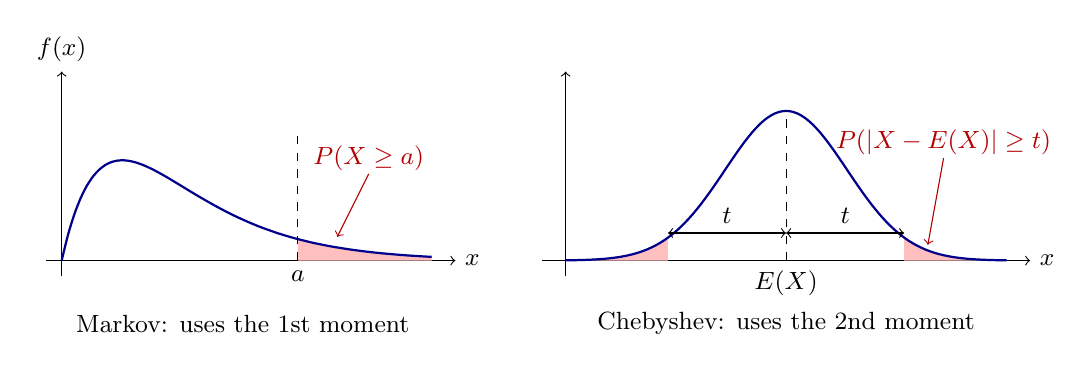
\begin{tikzpicture}[scale=1, every node/.style={font=\small}]
    % Markov: non-negative density, right tail beyond a
    \draw[->] (-0.2,0) -- (5,0) node[right]{$x$};
    \draw[->] (0,-0.2) -- (0,2.4) node[above]{$f(x)$};
    \fill[red!25, domain=3:4.7, variable=\x] (3,0) -- plot ({\x}, {3*\x*exp(-1.3*\x)*1.5}) -- (4.7,0) -- cycle;
    \draw[thick, blue!55!black, domain=0:4.7, smooth, samples=60, variable=\x] plot ({\x}, {3*\x*exp(-1.3*\x)*1.5});
    \draw[dashed] (3,0) -- (3,1.6);
    \node[below] at (3,0) {$a$};
    \node[red!70!black] at (3.9,1.3) {$P(X \geq a)$};
    \draw[->, red!70!black] (3.9,1.1) -- (3.5,0.3);
    \node at (2.3,-0.8) {\text{Markov: uses the 1st moment}};
    % Chebyshev: bell curve, both tails beyond E(X) +- t
    \begin{scope}[xshift=7.3cm]
        \draw[->] (-1.2,0) -- (5,0) node[right]{$x$};
        \draw[->] (-0.9,-0.2) -- (-0.9,2.4);
        \fill[red!25, domain=3.4:4.7, variable=\x] (3.4,0) -- plot ({\x}, {1.9*exp(-0.5*(\x-1.9)^2/0.6)}) -- (4.7,0) -- cycle;
        \fill[red!25, domain=-0.9:0.4, variable=\x] (-0.9,0) -- plot ({\x}, {1.9*exp(-0.5*(\x-1.9)^2/0.6)}) -- (0.4,0) -- cycle;
        \draw[thick, blue!55!black, domain=-0.9:4.7, smooth, samples=60, variable=\x] plot ({\x}, {1.9*exp(-0.5*(\x-1.9)^2/0.6)});
        \draw[dashed] (1.9,0) -- (1.9,1.9);
        \node[below] at (1.9,0) {$E(X)$};
        \draw[<->] (1.9,0.35) -- node[above]{$t$} (3.4,0.35);
        \draw[<->] (0.4,0.35) -- node[above]{$t$} (1.9,0.35);
        \node[red!70!black] at (3.9,1.5) {$P(|X-E(X)| \geq t)$};
        \draw[->, red!70!black] (3.9,1.3) -- (3.7,0.2);
        \node at (1.9,-0.8) {\text{Chebyshev: uses the 2nd moment}};
    \end{scope}
\end{tikzpicture}
\end{center}
\begin{center}
    "Concentration of Probability Mass"
\end{center}
Where Markov uses the 1st moment, Chebyshev uses 2nd moment.
\\What if we use other transformation/moments to quantify the tail probability?
\\E.g. the exponential moment? $\Rightarrow$ Chernoff's Inequality
\[M_X(t) = E[e^{tX}]\]

\begin{theorem}[Chernoff's Inequality][4.3]
    For all $t\geq 0$, \quad $P(X\geq E(X) + t) \leq \inf_{\lambda>0}M_{X - E(X)} (\lambda)e^{-\lambda t}$
    \[P(X\geq E(X) + t) \text{ roughly } P(\underbrace{X-E(X)}_{\substack{\text{distance between $X$} \\ \text{to its expected value}}}\geq t)\]
    \[\leq \inf_{\lambda>0} M_{X-E(X)} (\lambda)e^{-\lambda t}\]
    \begin{proof}
        the function $g(x) = e^x$ is monotonically increasing and non-negative.
        \[P(X-E(X) \geq t)\]
        \[=P(e^{X-E(X)} \geq e^t)\]
        \[=P(e^{\lambda(X-E(X))}\geq e^{\lambda t}) \quad \lambda > 0\]
        Since $e^{\lambda(X-E(X))} \geq 0$ a.s., we can apply Markov's inequality
        \[\leq \frac{E[e^{\lambda (X - E(X))}]}{e^{\lambda t}} \quad \text{where the numerator is the mgf } M_{X-E(X)}(\lambda)\]
        We proved that
        \[P(X-E(X) \geq t) \leq e^{-\lambda t} \cdot M_{X-E(X)}(\lambda)\]
        Since this inequality holds for any arbitrary $\lambda > 0$, we can take the inf:
        \[P(X-E(X) \geq t) \leq \inf_{\lambda>0}e^{-\lambda t}M_{X-E(X)}(\lambda)\]
        \hfill $\square$
    \end{proof}
\end{theorem}

\subsection{Hoeffding's Inequality (Thm 4.4)}

\begin{definition}[Convex Function][4.4.1]
    A function $f: \mathbb{R} \to \mathbb{R}$ is convex if for all $\lambda \in (0,1)$ and $x,y \in \mathbb{R}$
    \[f(\lambda x+(1-\lambda)y) \leq \lambda f(x)+ (1-\lambda)f(y)\]
    Any value between $x$ and $y$ can be represented as
    \[\lambda x+ (1-\lambda)y \text{ for } \lambda \in (0,1)\]
    \begin{center}
    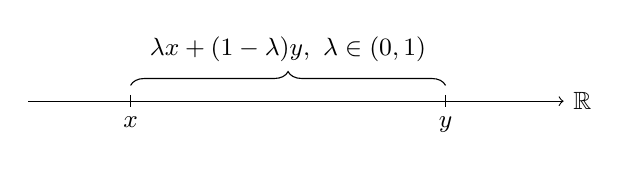
\begin{tikzpicture}[scale=1, every node/.style={font=\small}]
        \draw[->] (-0.3,0) -- (6.5,0) node[right]{$\mathbb{R}$};
        \draw (1,0.08) -- (1,-0.08) node[below]{$x$};
        \draw (5,0.08) -- (5,-0.08) node[below]{$y$};
        \draw[decorate, decoration={brace, amplitude=5pt}] (1,0.2) -- (5,0.2)
            node[midway, above=5pt]{\text{$\lambda x + (1-\lambda)y,\ \lambda \in (0,1)$}};
    \end{tikzpicture}
    \end{center}
    if $\lambda \to 1$, then the value is closer to $x$. Vice versa for $\lambda \to 0$, the value is closer to $y$.
    \begin{center}
    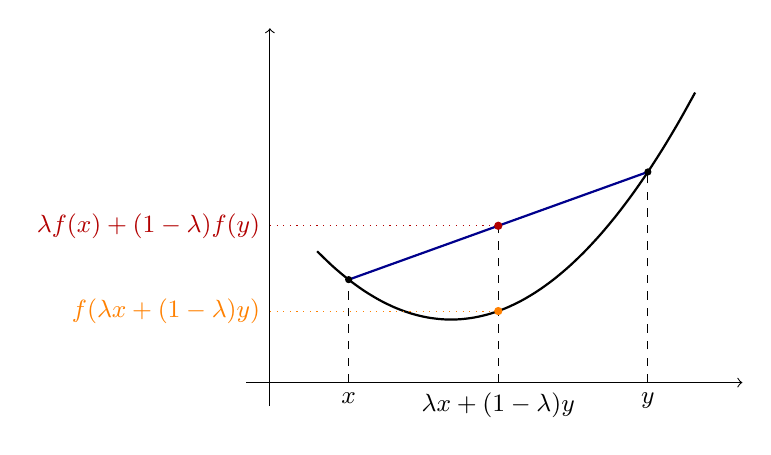
\begin{tikzpicture}[scale=1, every node/.style={font=\small}]
        \draw[->] (-0.3,0) -- (6,0);
        \draw[->] (0,-0.3) -- (0,4.5);
        \draw[thick, domain=0.6:5.4, smooth, variable=\x] plot ({\x}, {0.3*(\x-2.3)^2+0.8});
        % chord between x=1 and y=4.8
        \coordinate (A) at (1, {0.3*(1-2.3)^2+0.8});
        \coordinate (B) at (4.8, {0.3*(4.8-2.3)^2+0.8});
        \draw[thick, blue!55!black] (A) -- (B);
        \fill (A) circle (1.3pt); \fill (B) circle (1.3pt);
        % point lambda x + (1-lambda) y at x = 2.9 (lambda = 1/2)
        \coordinate (C) at (2.9, 1.991);
        \coordinate (F) at (2.9, {0.3*(2.9-2.3)^2+0.8});
        \draw[dashed] (1,0) -- (A);
        \draw[dashed] (4.8,0) -- (B);
        \draw[dashed] (2.9,0) -- (C);
        \draw[dotted, red!70!black] (0,0 |- C) -- (C);
        \draw[dotted, orange] (0,0 |- F) -- (F);
        \fill[red!70!black] (C) circle (1.5pt);
        \fill[orange] (F) circle (1.5pt);
        \node[below] at (1,0) {$x$};
        \node[below] at (2.9,0) {$\lambda x + (1-\lambda)y$};
        \node[below] at (4.8,0) {$y$};
        \node[anchor=east, red!70!black] at (0,0 |- C) {$\lambda f(x) + (1-\lambda)f(y)$};
        \node[anchor=east, orange] at (0,0 |- F) {$f(\lambda x + (1-\lambda)y)$};
    \end{tikzpicture}
    \end{center}
    Convexity: $f(\lambda x+ (1-\lambda)y) \leq \lambda f(x) + (1-\lambda)f(y)$
    \\ \text{$\Rightarrow$ the function is under the straight line}
\end{definition}

\begin{lemma}[Hoeffding's Lemma][4.4.2]
    If $Y$ satisfies $E(Y) = 0$ and $a\leq Y \leq b$ a.s., then for all $\lambda > 0$
    \[M_Y(\lambda) \leq e^{\lambda^2(b-a)^2/8}\]
    \begin{proof}
        Since $a \leq Y \leq b$ a.s., $Y = \alpha \cdot a + (1-\alpha)\cdot b$.
        \\ Transforming $Y \Rightarrow \alpha$, where $0 \leq \alpha \leq 1$,
        \[\alpha = \frac{b-Y}{b-a}, \qquad 1-\alpha = \frac{Y-a}{b-a}\]
        Also, since the function $e^{\lambda y}$ is convex,
        \[e^{\lambda(\alpha a + (1-\alpha)b)} \leq \alpha e^{\lambda a} + (1-\alpha)e^{\lambda b}\]
        Apply $f(y) = e^{\lambda y}$ transformation to r.v.\ $Y$:
        \[e^{\lambda Y} \leq \alpha e^{\lambda a} + (1-\alpha)e^{\lambda b} = \frac{b-Y}{b-a}e^{\lambda a} + \frac{Y-a}{b-a}e^{\lambda b}\]
        Take expectation on both sides:
        \[E[e^{\lambda Y}] \leq E\Big[\frac{b-\overbrace{Y}^{\text{random var.}}}{b-a}\underbrace{e^{\lambda a}}_{\text{constant}}\Big] + E\Big[\frac{Y-a}{b-a}\underbrace{e^{\lambda b}}_{\text{constant}}\Big]\]
        \[= \frac{b-E(Y)}{b-a}e^{\lambda a} + \frac{E(Y)-a}{b-a}e^{\lambda b}\]
        \[= \underbrace{\frac{b}{b-a}}_{p}e^{\lambda a} + \frac{-a}{b-a}e^{\lambda b} \qquad (\text{since } E(Y) = 0)\]
        Next, we let $p = \frac{b}{b-a}$:
        \[E[e^{\lambda Y}] \leq pe^{\lambda a} + (1-p)e^{\lambda b}\]
        We take log on RHS:
        \[\log\{E[e^{\lambda Y}]\} \leq \log\{pe^{\lambda a} + (1-p)e^{\lambda b}\}\]
        \[= \log\{e^{\lambda a}[p + (1-p)e^{\lambda(b-a)}]\}\]
        \[= \underbrace{\lambda a}_{\textcolor{blue!55!black}{=(p-1)u}} + \log[p + (1-p)e^{\lambda(b-a)}]\]
        \[\textcolor{blue!55!black}{(p-1)u = \left(\frac{b}{b-a}-1\right)(b-a)\lambda = \frac{a}{b-a}(b-a)\lambda = a\lambda}\]
        Next, let $u = (b-a)\lambda$:
        \[\log\{E[e^{\lambda Y}]\} \leq (p-1)u + \log[p + (1-p)e^u] =: \varphi(u)\]
        \[\varphi(0) = 0, \qquad \varphi'(u) = (p-1) + \frac{(1-p)e^u}{p+(1-p)e^u}, \qquad \varphi'(0) = 0\]
        \[\varphi(u) = \underbrace{\varphi(0)}_{0} + \underbrace{\varphi'(0)}_{0}u + \frac{1}{2}\varphi''(\xi)u^2 \qquad \text{(Taylor's Expansion at } u = 0)\]
        For some $\xi$ between $0$ and $u$, \quad $\varphi(u) = \frac{1}{2}\varphi''(\xi)u^2$
        \[\varphi''(u) = \frac{p(1-p)e^u}{[p+(1-p)e^u]^2} \leq \frac{1}{4}\]
        \[\Rightarrow \varphi(u) \leq \frac{1}{8}u^2\]
        \[\Rightarrow \log\{E[e^{\lambda Y}]\} \leq \frac{1}{8}u^2 = \frac{(b-a)^2\lambda^2}{8} \quad \text{as } u = (b-a)\lambda\]
        \[\Rightarrow M_Y(\lambda) \leq e^{\frac{(b-a)^2\lambda^2}{8}}\]
        \hfill $\square$
    \end{proof}
\end{lemma}

\begin{theorem}[Hoeffding's Inequality][4.4]
    Suppose $X_1, X_2, \dots, X_n, \dots$ are indep.\ with $a_i \leq X_i \leq b_i$ for all $i$.
    \\ Then letting $S_n = \sum_{i=1}^n X_i$, for all $t > 0$,
    \[P(|S_n - E(S_n)| \geq t) \leq 2 \cdot \exp\left\{-\frac{2t^2}{\sum_{i=1}^n (b_i - a_i)^2}\right\}\]
    \begin{proof}
        We first prove the $P(S_n - E(S_n) \geq t)$ part.
        \\ Applying Chernoff's inequality,
        \[P(\underbrace{S_n - E(S_n)}_{(1)} \geq t) \leq e^{-\lambda t}\underbrace{E[e^{\lambda(S_n - E(S_n))}]}_{(2)}\]
        (1): \quad $S_n - E(S_n) = \sum_{i=1}^n (X_i - E(X_i))$ \quad as $S_n = \sum_{i=1}^n X_i$
        \\ (2): \[e^{\lambda(S_n - E(S_n))} = e^{\lambda\sum_{i=1}^n (X_i - E(X_i))} = \prod_{i=1}^n e^{\lambda[X_i - E(X_i)]}\]
        Taking expectations, the factors are independent so $E$ of the product $=$ product of $E$'s:
        \[M_{S_n - E(S_n)}(\lambda) = \prod_{i=1}^n M_{X_i - E(X_i)}(\lambda)\]
        Applying Hoeffding's Lemma to $Y = X_i - E(X_i)$: \quad $M_{X_i - E(X_i)}(\lambda) \leq e^{\frac{(b_i - a_i)^2\lambda^2}{8}}$
        \[M_{S_n - E(S_n)}(\lambda) \leq \prod_{i=1}^n e^{\frac{(b_i-a_i)^2\lambda^2}{8}} = e^{\frac{\lambda^2}{8}\sum_{i=1}^n (b_i - a_i)^2}\]
        Combine with Chernoff's inequality:
        \[P(S_n - E(S_n) \geq t) \leq e^{-\lambda t + \frac{\lambda^2}{8}\sum_{i=1}^n (b_i - a_i)^2}\]
        Rearrange, we have Hoeffding's inequality.
        \hfill $\square$
    \end{proof}
\end{theorem}

% !TeX root = ../main.tex

\newlecture[Jensen, Young, H\"older and Minkowski Inequalities][Oct 1, 2026]

\begin{reqproof}
\begin{theorem}[Jensen's Inequality][4.5]\req{t4.5}\reqtoc{t4.5}{Thm 4.5 Jensen's Inequality}
    If $f$ is a convex function and $X$ is a random variable such that $f(X)$ is integrable,
    \[f(EX) \leq Ef(X)\]
    The inequality is \dbb{flipped} if $f$ is \dbb{concave}.
    \begin{proof}
    Since $f$ is convex, there exists a function $g$ s.t.
    \begin{align*}
        g(x) &= ax + b \text{ and} & &\db{\Leftarrow \quad g(\cdot) \text{ is a straight line}}\\
        g(x) &\leq f(x) \text{ for all }x \text{ and} & &\db{\Leftarrow \quad g(\cdot) \text{ always below }f(\cdot)}\\
        g(EX) &= f(EX) & &\db{\Leftarrow \quad g(\cdot)=f(\cdot) \text{ at } x=EX}
    \end{align*}
    \begin{center}
    \begin{tikzpicture}[scale=1, every node/.style={font=\small}]
        \draw[->] (-0.2,0) -- (5,0) node[right]{$x$};
        \draw[->] (0,-0.2) -- (0,3.6);
        \draw[thick, domain=0.5:4.3, smooth, variable=\x] plot ({\x}, {0.35*(\x-1.8)^2+1});
        \draw[thick, blue!55!black] (0,0.2825) -- (4.7,1.9275);
        \fill (2.3,1.0875) circle (1.5pt);
        \draw[dotted] (2.3,0) -- (2.3,1.0875);
        \draw[dotted] (0,1.0875) -- (2.3,1.0875);
        \node[below] at (2.3,0) {$E(X)$};
        \node[left, blue!55!black] at (0,1.0875) {$g(EX) = f(EX)$};
        \node[anchor=west] at (4.3,3.2) {$f(\cdot)$};
        \node[anchor=west, blue!55!black] at (4.75,1.93) {\text{$g(\cdot)$: straight, always below $f(\cdot)$}};
    \end{tikzpicture}
    \end{center}
    \[f(x) \geq g(x) \text{ for all }x\]
    \begin{align*}
        E[f(X)] \geq E[g(X)] &= E[aX+b]\\
        &= aE(X)+b\\
        &= g(E(X))\\
        &= f(E(X))
    \end{align*}
    \end{proof}
\end{theorem}
\end{reqproof}

\begin{example}[Applying the Jensen's Inequality][4.5.1]
    \[[E(X)]^2 \leq E[X^2] \quad f(x) = x^2 \Rightarrow \text{convex}\]
    \[E[\log X] \leq \log [EX] \quad f(x) = \log x \Rightarrow \text{concave}\]
\end{example}

\begin{reqproof}
\begin{lemma}[Young's Inequality][4.6]\req{l4.6}\reqtoc{l4.6}{Lemma 4.6 Young's Inequality}
    For any $p, q > 1$ and $\frac{1}{p}+ \frac{1}{q} = 1$,
    \[xy \leq \frac{x^p}{p} + \frac{y^q}{q} \quad \text{for any }x,y \geq 0 \]
    \begin{proof}
    Let $h_y(x) = \frac{1}{p}x^p + \frac{1}{q}y^q -xy$
    \\To prove $h_y(x) \geq 0$, we take derivatives
    \[h_y'(x) = \frac{dh_y(x)}{dx} = x^{p-1} - y\]
    \[h_y''(x) = \frac{d^2h_y(x)}{dx^2} = (p-1)x^{p-2} \geq 0, \text{ because } x \geq 0\]
    Therefore $h_y'(x) = 0 \Rightarrow x^* = y^{\frac{1}{p-1}}$ is the minimizer.
    \\Plugging in,
    \begin{align*}
        h_y(x^*) &= \frac{1}{p}\left(y^{\frac{1}{p-1}}\right)^p + \frac{1}{q}y^q - y^{\frac{1}{p-1}} \cdot y\\
        &= \frac{1}{p}y^{\frac{p}{p-1}} + \frac{1}{q}y^q - y^{\frac{p}{p-1}}
    \end{align*}
    Since
    \[\frac{1}{p}+\frac{1}{q} = 1 \;\Rightarrow\; \frac{1}{q} = 1 - \frac{1}{p} \;\Rightarrow\; q = \frac{p}{p-1}\]
    substituting $q = \frac{p}{p-1}$ and $\frac{1}{q} = 1 - \frac{1}{p}$:
    \begin{align*}
        h_y(x^*) &= \frac{1}{p}y^{\frac{p}{p-1}} + \left(1-\frac{1}{p}\right)y^{\frac{p}{p-1}} - y^{\frac{p}{p-1}}\\
        &= 0
    \end{align*}
    \[\Rightarrow h_y(x) \geq h_y(x^*) = 0\]
    Therefore $\frac{1}{p}x^p + \frac{1}{q}y^q \geq xy$.
    \\(If $p=q=2$: $\frac{1}{2}x^2 + \frac{1}{2}y^2 \geq xy \;\Leftrightarrow\; x^2+y^2 \geq 2xy$.)
    \end{proof}
\end{lemma}
\end{reqproof}

\begin{reqproof}
\begin{theorem}[H\"older's Inequality][4.6]\req{t4.6}\reqtoc{t4.6}{Thm 4.6 \texorpdfstring{H\"older}{Hölder}'s Inequality}
    If $p,q > 1$ s.t. $\frac{1}{p} + \frac{1}{q} = 1$,
    \[E[|XY|] \leq [E(|X|^p)]^{\frac{1}{p}} \cdot [E(|Y|^q)]^{\frac{1}{q}}\]

    \begin{proof}
    Let
    \[X^* = \frac{|X|}{[E(|X|^p)]^{\frac{1}{p}}} \quad \text{and} \quad Y^* = \frac{|Y|}{[E(|Y|^q)]^{\frac{1}{q}}}\]
    Observe that
    \[E[(X^*)^p] = E[(Y^*)^q] = 1\]
    since
    \[E[(X^*)^p] = E\left[\left(\frac{|X|}{[E(|X|^p)]^{\frac{1}{p}}}\right)^p\right] = E\left[\frac{|X|^p}{E(|X|^p)}\right] = \frac{E(|X|^p)}{E(|X|^p)} = 1\]
    and the same for $Y^*$ with $q$.

    Applying the Young's Inequality
    \[X^*Y^* \leq \frac{(X^*)^p}{p} + \frac{(Y^*)^q}{q}\]
    Take expectations on both sides
    \[E[X^*Y^*]\leq \frac{E[(X^*)^p]}{p} + \frac{E[(Y^*)^q]}{q}\]
    \[E\left[\frac{|X||Y|}{E(|X|^p)^{\frac{1}{p}}E(|Y|^q)^{\frac{1}{q}}}\right] \leq \frac{1}{p}+ \frac{1}{q} = 1\]
    Therefore, re-arrange
    \[E[|X||Y|] \leq E(|X|^p)^{\frac{1}{p}} E(|Y|^q)^{\frac{1}{q}}\]
    \end{proof}
\end{theorem}
\end{reqproof}

\begin{reqproof}
\begin{proposition}[Cauchy-Schwarz Inequality][4.6.1]\req{p4.6.1}\reqtoc{p4.6.1}{Prop 4.6.1 Cauchy-Schwarz Inequality}
    \[E[|XY|] \leq \sqrt{E(X^2)E(Y^2)}\]
    \begin{proof}
    Exercise.
    \end{proof}
\end{proposition}
\end{reqproof}

\begin{reqnoproof}
\begin{theorem}[Minkowski's Inequality][4.7]\req{t4.7}\reqtoc{t4.7}{Thm 4.7 Minkowski's Inequality}
    If $p>1$, then
    \[[E(|X+Y|^p)]^{\frac{1}{p}} \leq [E(|X|^p)]^{\frac{1}{p}} + [E(|Y|^p)]^{\frac{1}{p}}\]
    \begin{center}
        (The triangle inequality in probability)
    \end{center}
\end{theorem}
\end{reqnoproof}

{\large\rb{EXAM UPDATE: CAN BRING CHEATSHEET DOUBLE SIDE HANDWRITTEN!!!!}\par}

\chapterentry{Chapter 5: Limiting Theorems and Convergences}
% !TeX root = ../main.tex

\newlecture[Continuity of Measure, Tail Events and Borel-Cantelli][Oct 6, 2026]

\begin{reqproof}
\begin{theorem}[Continuity of Measure][5.1]\req{t5.1}\reqtoc{t5.1}{Thm 5.1 Continuity of Measure}
    If $\left\{A_n\right\} \uparrow A$ or $\left\{A_n\right\} \downarrow A$, then $\lim_{n\to \infty} P(A_n) = P(A)$.
    \\Note:
    \begin{enumerate}
        \item $\left\{A_n\right\} \uparrow A$ means:
        \[A_1 \subseteq A_2 \subseteq \cdots \subseteq A_n \subseteq \cdots \to A, \qquad \lim_{n\to \infty} \bigcup_{i=1}^n A_i = A\]
        \item $\left\{A_n\right\}\downarrow A$ means:
        \[A_1 \supseteq A_2 \supseteq \cdots \supseteq A_n \supseteq \cdots \to A, \qquad \lim_{n\to \infty} \bigcap_{i=1}^n A_i = A\]
    \end{enumerate}
    Note: $A_1 \subseteq \cdots \subseteq A_n \subseteq \cdots \to A$ means
    \[P(A_1) \leq \cdots \leq P(A_n) \leq \cdots \to P(A)\]
    \begin{proof}
        Suppose $\left\{A_n\right\} \uparrow A$.
        \\We let $A_0 = \varnothing$, and $B_1 = A_1$, $B_n = A_n \cap A_{n-1}^c$.
        \begin{center}
        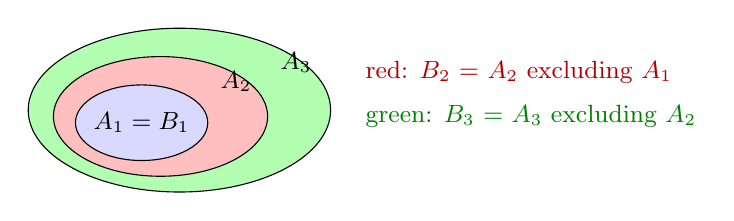
\begin{tikzpicture}[scale=0.8, every node/.style={font=\small}]
            \fill[green!30] (0,0) ellipse (2.4cm and 1.3cm);
            \fill[red!25] (-0.3,-0.1) ellipse (1.7cm and 0.95cm);
            \fill[blue!15] (-0.6,-0.2) ellipse (1.05cm and 0.6cm);
            \draw (0,0) ellipse (2.4cm and 1.3cm);
            \draw (-0.3,-0.1) ellipse (1.7cm and 0.95cm);
            \draw (-0.6,-0.2) ellipse (1.05cm and 0.6cm);
            \node at (-0.6,-0.2) {$A_1 = B_1$};
            \node at (0.9,0.45) {$A_2$};
            \node at (1.85,0.75) {$A_3$};
            \node[anchor=west, red!70!black] at (2.8,0.6) {red: $B_2$ = $A_2$ excluding $A_1$};
            \node[anchor=west, green!50!black] at (2.8,-0.1) {green: $B_3$ = $A_3$ excluding $A_2$};
        \end{tikzpicture}
        \end{center}
        Observe that:
        \begin{enumerate}
            \item $\bigcup_{i=1}^n A_i = \bigcup_{i=1}^n B_i$
            \item $B_i$'s are disjoint.
        \end{enumerate}
        Therefore, $P\left(\bigcup_{i=1}^n A_i\right) = P\left(\bigcup_{i=1}^n B_i\right)$, and
        \begin{align*}
            P(A) = P\left(\lim_{n\to\infty}\bigcup_{i=1}^n A_i\right) &= P\left(\lim_{n\to\infty}\bigcup_{i=1}^n B_i\right) = P\left(\bigcup_{i=1}^\infty B_i\right)\\
            &= \lim_{n\to\infty}\sum_{i=1}^n P(B_i)\\
            &= \lim_{n\to\infty} P(A_n)
        \end{align*}
        For the case $A_n \downarrow A$, the proof is similar; one may take the complement:
        \[\left\{A_n\right\}\downarrow A \;\Rightarrow\; \left\{A_n^c\right\}\uparrow A^c\]
    \end{proof}
\end{theorem}
\end{reqproof}

\begin{example}[][5.1.1]
    If each $A_n = \left[0, 1-\frac{1}{n}\right]$, then
    \[\lim_{n\to\infty} A_n = [0,1) = A, \qquad A_n \uparrow A\]
    If we apply a uniform measure $P(\cdot)$ on $\left\{A_n\right\}$,
    \[P(A) = \lim_{n\to\infty} P(A_n) = \lim_{n\to\infty}\left(1-\frac{1}{n}\right) = 1\]
\end{example}

\begin{reqproof}
\begin{definition}[Tail Events][5.2]\req{d5.2}\reqtoc{d5.2}{Def 5.2 Tail Events}
    Consider a sequence $A_1, A_2, \dots \subseteq \Omega$, define the tail events as:
    \[\limsup_{n\to\infty} A_n = \left\{A_n \text{ i.o.}\right\} = \bigcap_{n=1}^\infty \bigcup_{k=n}^\infty A_k\]
    \[\liminf_{n\to\infty} A_n = \left\{A_n \text{ a.a.}\right\} = \bigcup_{n=1}^\infty \bigcap_{k=n}^\infty A_k\]
    Note: the notations
    \\ i.o.\ means \dbb{infinitely often}
    \\ a.a.\ means \dbb{almost always}
\end{definition}
\end{reqproof}

\[\limsup_{n\to\infty} A_n = \left\{A_n \text{ i.o.}\right\} = \bigcap_{n=1}^\infty \underbrace{\bigcup_{k=n}^\infty A_k}_{\text{tail union}}\]
You want to find the smallest set that contains the union of your tail events:
\\``elements that will appear infinitely many times''.
\[\liminf_{n\to\infty} A_n = \left\{A_n \text{ a.a.}\right\} = \bigcup_{n=1}^\infty \underbrace{\bigcap_{k=n}^\infty A_k}_{\text{tail intersect}}\]
You want to find the largest set that contains the intersect of your tail events:
\\``elements that will appear in all tail sets''.

\begin{example}[Tail Events][\relax]
    Suppose $\left\{A_n\right\}$ is constructed as follows:
    \[A_i = \begin{cases}
        \left\{\textcolor{blue}{\text{blue}}, \textcolor{red}{\text{red}}\right\} & i \text{ odd}\\
        \left\{\textcolor{blue}{\text{blue}}, \textcolor{green!60!black}{\text{green}}, \textcolor{orange}{\text{orange}}\right\} & i \text{ even}
    \end{cases}\]
    \begin{center}
    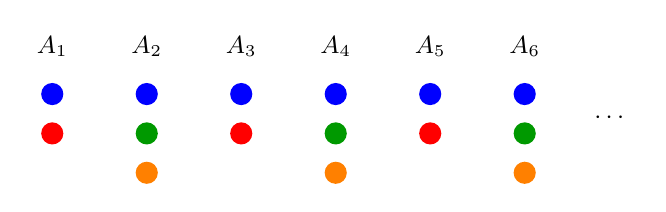
\begin{tikzpicture}[scale=1, every node/.style={font=\small}]
        \foreach \i in {1,...,6} {
            \node at (1.2*\i,0.6) {$A_{\i}$};
            \fill[blue] (1.2*\i,0) circle (4pt);
        }
        \foreach \i in {1,3,5} \fill[red] (1.2*\i,-0.5) circle (4pt);
        \foreach \i in {2,4,6} {
            \fill[green!60!black] (1.2*\i,-0.5) circle (4pt);
            \fill[orange] (1.2*\i,-1.0) circle (4pt);
        }
        \node at (8.3,-0.3) {$\cdots$};
    \end{tikzpicture}
    \end{center}
    \[\limsup_{n\to\infty} A_n = \left\{A_n \text{ i.o.}\right\} = \left\{\textcolor{blue}{\text{blue}}, \textcolor{red}{\text{red}}, \textcolor{green!60!black}{\text{green}}, \textcolor{orange}{\text{orange}}\right\}\]
    \[\liminf_{n\to\infty} A_n = \left\{A_n \text{ a.a.}\right\} = \left\{\textcolor{blue}{\text{blue}}\right\}\]
    $\left\{A_n \text{ i.o.}\right\} \Rightarrow$ ``the elements that will appear infinitely often in the tail of $\left\{A_n\right\}$''
    \\$\left\{A_n \text{ a.a.}\right\} \Rightarrow$ ``the elements that will appear almost always in the tail of $\left\{A_n\right\}$''
\end{example}

\begin{reqproof}
\begin{corollary}[][5.2.1]\req{c5.2.1}\reqtoc{c5.2.1}{Corollary 5.2.1}
    \[P(A_n \text{ i.o.}) = 1 - P(A_n^c \text{ a.a.})\]
\end{corollary}
\end{reqproof}

\begin{reqproof}
\begin{proposition}[][5.2.2]\req{p5.2.2}\reqtoc{p5.2.2}{Prop 5.2.2}
    \[P(A_n \text{ a.a.}) \leq \liminf_{n\to\infty} P(A_n) \leq \limsup_{n\to\infty} P(A_n) \leq P(A_n \text{ i.o.})\]
    i.e.
    \[P\left(\liminf_{n\to\infty} A_n\right) \leq \liminf_{n\to\infty} P(A_n) \leq \limsup_{n\to\infty} P(A_n) \leq P\left(\limsup_{n\to\infty} A_n\right)\]
    \begin{proof}
        We prove the 1st ``$\leq$''.
        \[\liminf_{n\to\infty} A_n = \bigcup_{n=1}^\infty \underbrace{\bigcap_{k=n}^\infty A_k}_{B_n}\]
        We let $B_n = \bigcap_{k=n}^\infty A_k$ (``the intersect of tail events''), so $\liminf_{n\to\infty} A_n = \bigcup_{n=1}^\infty B_n$.
        \\Notice that $B_1 \subseteq B_2 \subseteq \cdots \subseteq B_n \subseteq \cdots$ as $B_n = \bigcap_{k=n}^\infty A_k$:
        \begin{align*}
            B_1 &= A_1 \cap A_2 \cap \cdots \cap A_n \cap \cdots\\
            B_2 &= \phantom{A_1 \cap{}} A_2 \cap \cdots \cap A_n \cap \cdots \qquad \Rightarrow B_1 \subseteq B_2
        \end{align*}
        So $B_n \uparrow B = \bigcup_{n=1}^\infty B_n$, and $\lim_{n\to\infty} P(B_n) = P(B)$ by continuity of measure (Thm 5.1).
        \begin{align*}
            P\left(\liminf_{n\to\infty} A_n\right) &= P\left(\bigcup_{n=1}^\infty B_n\right) = P\left(\lim_{n\to\infty} B_n\right)\\
            &= \lim_{n\to\infty} P(B_n) & &\text{as $B_n$ converges}\\
            &= \liminf_{n\to\infty} P(B_n) = \liminf_{n\to\infty} P\left(\bigcap_{k=n}^\infty A_k\right)\\
            &\leq \liminf_{n\to\infty} P(A_n) & &\text{because } \textstyle\bigcap_{k=n}^\infty A_k \subseteq A_n
        \end{align*}
        The 2nd ``$\leq$'' is by definition.
        \\The 3rd ``$\leq$'' can be proved similarly.
    \end{proof}
\end{proposition}
\end{reqproof}

\begin{reqnoproof}
\begin{theorem}[Borel-Cantelli Lemma][5.3]\req{t5.3}\reqtoc{t5.3}{Thm 5.3 Borel-Cantelli Lemma}
    \begin{enumerate}[label=\roman*)]
        \item If $\sum_{n=1}^\infty P(A_n) < \infty$, then $P(A_n \text{ i.o.}) = 0$.
        \item If $\sum_{n=1}^\infty P(A_n) = \infty$ and $\left\{A_n\right\}$ are independent, then $P(A_n \text{ i.o.}) = 1$.
    \end{enumerate}
    \begin{proof}
        \begin{enumerate}[label=\roman*)]
            \item
            \[\left\{A_n \text{ i.o.}\right\} = \bigcap_{n=1}^\infty \underbrace{\bigcup_{k=n}^\infty A_k}_{B_n}, \qquad B_n = \bigcup_{k=n}^\infty A_k, \qquad B_n \downarrow B\]
            \begin{align*}
                P(A_n \text{ i.o.}) &= P\left(\bigcap_{n=1}^\infty\bigcup_{k=n}^\infty A_k\right) = P\left(\bigcap_{n=1}^\infty B_n\right)\\
                &= \lim_{n\to\infty} P(B_n) & &\text{as } B_n \downarrow B = \textstyle\bigcap_{n=1}^\infty B_n\\
                &= \lim_{n\to\infty} P\left(\bigcup_{k=n}^\infty A_k\right)\\
                &\leq \lim_{n\to\infty} \sum_{k=n}^\infty P(A_k)\\
                &= 0 & &\text{as } \textstyle\sum_{k=1}^\infty P(A_k) < \infty
            \end{align*}

            \item
            \begin{align*}
                1 - P(A_n \text{ i.o.}) &= P\left(\left\{A_n \text{ i.o.}\right\}^c\right)\\
                &= P\left(\bigcup_{n=1}^\infty \underbrace{\bigcap_{k=n}^\infty A_k^c}_{C_n}\right) & &\text{because } \left\{A_n \text{ i.o.}\right\}^c = \textstyle\bigcup_{n=1}^\infty\bigcap_{k=n}^\infty A_k^c
            \end{align*}
            Let $C_n = \bigcap_{k=n}^\infty A_k^c$, $C_n \uparrow C$.
            \begin{align*}
                &= P\left(\bigcup_{n=1}^\infty C_n\right) = P\left(\lim_{n\to\infty} C_n\right) & &\text{as } C_n \uparrow C\\
                &= \lim_{n\to\infty} P(C_n) = \lim_{n\to\infty} P\left(\bigcap_{k=n}^\infty A_k^c\right)\\
                &= \lim_{n\to\infty}\prod_{k=n}^\infty \left[1 - P(A_k)\right] & &\text{because $\{A_n\}$ independent}
            \end{align*}
            \\Each factor $1 - P(A_k) \leq 1$, but that alone doesn't give $0$. The missing step: use $1 - x \leq e^{-x}$:
            \[\prod_{k=n}^\infty\left[1 - P(A_k)\right] \leq \prod_{k=n}^\infty e^{-P(A_k)} = \exp\left\{-\sum_{k=n}^\infty P(A_k)\right\} = e^{-\infty} = 0\]
            since $\sum_{k=n}^\infty P(A_k) = \infty$ for every $n$. So
            \[1 - P(A_n \text{ i.o.}) = 0 \;\Rightarrow\; P(A_n \text{ i.o.}) = 1\]
        \end{enumerate}
    \end{proof}
\end{theorem}
\end{reqnoproof}

\begin{example}[Converse does NOT hold for i)][5.3.1]
    Uniform measure and $A_n = \left[0, \frac{1}{n}\right]$. Then $A_n \downarrow A = \left\{0\right\}$, and
    \begin{align*}
        \left\{A_n \text{ i.o.}\right\} &= \bigcap_{n=1}^\infty\bigcup_{k=n}^\infty A_k = \bigcap_{n=1}^\infty\bigcup_{k=n}^\infty\left[0, \frac{1}{k}\right]\\
        &= \left\{0\right\} = \lim_{n\to\infty} A_n
    \end{align*}
    \[P(\left\{A_n \text{ i.o.}\right\}) = P(\left\{0\right\}) = 0\]
    but
    \[\sum_{n=1}^\infty P(A_n) = \sum_{n=1}^\infty \frac{1}{n} = \infty\]
\end{example}

\begin{example}[Independence is needed for ii)][5.3.2]
    Define $C_1, C_2, \dots$ to be results of a fair coin toss, such that $C_i = 1$ if the $i$-th toss resulted in H.
    \\Let $A_1, A_2, \dots$ be events such that
    \[A_j = \left\{\text{the \hlt{1st} toss is H}\right\} \quad \text{for every } j\]
    Then
    \[\sum_{n=1}^\infty P(A_n) = \sum_{n=1}^\infty \frac{1}{2} = \lim_{n\to\infty}\frac{1}{2}\cdot n = \infty\]
    \[P(A_n \text{ i.o.}) = P(A_n) = \frac{1}{2} \neq 1\]
    as all $\left\{A_n\right\}$ are the same.
\end{example}

% !TeX root = ../main.tex

\newlecture[Convergence in Probability and Almost Sure Convergence][Oct 8, 2026]

\begin{reqproof}
\begin{definition}[Convergence in Probability][5.4]\req{d5.4}\reqtoc{d5.4}{Def 5.4 Convergence in Probability}
    A sequence of random variables $X_n$ converges in probability to $X$ if for all $\varepsilon > 0$
    \[\lim_{n\to \infty} P(\left|X_n - X\right| \leq \varepsilon) = 1 \qquad \text{or} \qquad \lim_{n\to \infty} P(\left|X_n - X\right| > \varepsilon) = 0\]
    and is denoted by $X_n \overset{P}{\longrightarrow} X$.
\end{definition}
\end{reqproof}

\begin{reqproof}
\begin{definition}[Almost Sure Convergence][5.5]\req{d5.5}\reqtoc{d5.5}{Def 5.5 Almost Sure Convergence}
    A sequence of random variables $X_n$ converges almost surely to $X$ if
    \[P(\lim_{n \to \infty} X_n = X) = 1\]
    and is denoted by $X_n \overset{a.s.}{\longrightarrow} X$.
\end{definition}
\end{reqproof}

\heading{Compare the two:}
\[X_n \overset{P}{\longrightarrow} X \qquad \lim_{n\to \infty} P(\left|X_n - X\right| < \varepsilon ) = 1\]
\[X_n \overset{a.s.}{\longrightarrow} X \qquad P(\lim_{n \to \infty} X_n = X) = 1\]
where
\[\lim_{n \to \infty} X_n = X \Leftrightarrow \left\{\omega: \lim_{n\to \infty} X_n (\omega) = X(\omega)\right\}\]
\[P(\lim_{n\to \infty} X_n = X) = P(\left\{\omega: \lim_{n \to \infty} X_n (\omega) = X(\omega)\right\})=1\]
Written in the same form, for all $\varepsilon > 0$:
\begin{align*}
    X_n &\overset{P}{\longrightarrow} X & &\lim_{n\to \infty} P(\left|X_n - X\right| < \varepsilon) = 1 \\
    X_n &\overset{a.s.}{\longrightarrow} X & &P(\left|X_n(\omega) - X(\omega)\right| < \varepsilon \text{ a.a.}) = 1
\end{align*}
``$\overset{a.s.}{\longrightarrow}$'' condition holds almost always: for intersect of the tail.
\\``$\overset{P}{\longrightarrow}$'' condition satisfied at target.

\begin{reqproof}
\begin{proposition}[][5.5.1]\req{p5.5.1}\reqtoc{p5.5.1}{Prop 5.5.1}
    If for all $\varepsilon > 0$, $P(\left|X_n - X\right| > \varepsilon \text{ i.o.}) = 0$, then
    \[X_n \overset{a.s.}{\longrightarrow} X\]
    \begin{proof}
        \begin{align*}
            P(\lim_{n\to \infty}X_n = X) &= P(\forall \varepsilon > 0,\ \left|X_n(\omega) - X(\omega)\right| < \varepsilon \text{ a.a.})\\
            &= 1-P(\left|X_n(\omega) - X(\omega)\right| \geq \varepsilon \text{ i.o.}) & &\text{(Corollary 5.2.1)}\\
            &= 1-0 = 1
        \end{align*}
    \end{proof}
\end{proposition}
\end{reqproof}

\begin{reqproof}
\begin{proposition}[][5.5.2]\req{p5.5.2}\reqtoc{p5.5.2}{Prop 5.5.2}
    If for all $\varepsilon > 0$,
    \[\sum_{n=1}^{\infty} P(\left|X_n(\omega) - X(\omega)\right| \geq \varepsilon) < \infty\]
    then $X_n \overset{a.s.}{\longrightarrow} X$.
    \begin{proof}
        Applying the Borel-Cantelli Lemma.
    \end{proof}
\end{proposition}
\end{reqproof}

\begin{reqproof}
\begin{proposition}[][5.5.3]\req{p5.5.3}\reqtoc{p5.5.3}{Prop 5.5.3}
    If $X_n \overset{a.s.}{\longrightarrow} X$, then $X_n \overset{P}{\longrightarrow}X$.
    \\The opposite doesn't hold: $X_n \overset{P}{\longrightarrow} X \nRightarrow X_n \overset{a.s.}{\longrightarrow} X$.
    \begin{proof}
        For any $\varepsilon > 0$, let
        \[E_n = \left\{\omega: \exists m \geq n,\ \left|X_m(\omega) - X(\omega)\right| \geq \varepsilon\right\}\]
        Observe that $E_{n+1} \subseteq E_n$, and if $\omega \in \bigcap_{n=1}^{\infty}E_n$ then $X_n(\omega) \overset{a.s.}{\not\longrightarrow} X(\omega)$.
        \begin{align*}
            \lim_{n\to \infty} P(\left|X_n(\omega) - X(\omega)\right|\geq \varepsilon) &\leq \lim_{n\to \infty} P(E_n)\\
            &= P\left(\bigcap_{n=1}^{\infty}E_n\right)\\
            &\leq P(\left\{\omega : X_n(\omega) \not\to X(\omega)\right\})\\
            &= 0 & &\text{since } X_n \overset{a.s.}{\longrightarrow} X
        \end{align*}
        So $\lim_{n\to\infty} P(|X_n - X| \geq \varepsilon) = 0$ for every $\varepsilon > 0$, i.e.\ $X_n \overset{P}{\longrightarrow} X$. The counterexample for the converse is Example 5.5.4.
    \end{proof}
\end{proposition}
\end{reqproof}

\begin{example}[][5.5.4]
    $X_n$ independent with $P(X_n = 1) = \frac{1}{n}$, $P(X_n = 0) = 1 - \frac{1}{n}$.
    \\For all $\varepsilon > 0$,
    \[P(X_n > \varepsilon) = \frac{1}{n} \to 0 \text{ as }n \to \infty\]
    \\So, $X_n \overset{P}{\longrightarrow} 0$.
    \\However,
    \[P(X_n = 1 \text{ i.o.}) = 1\]
    \[\Rightarrow X_n \overset{a.s.}{\not\longrightarrow} 0\]
\end{example}

\begin{reqnoproof}
\begin{theorem}[][5.5.5]\req{t5.5.5}\reqtoc{t5.5.5}{Thm 5.5.5}
    If $X_n \overset{P}{\longrightarrow} X$, there exists a subsequence such that
    \[X_{n_k} \overset{a.s.}{\longrightarrow} X\]
\end{theorem}
\end{reqnoproof}

\begin{reqnoproof}
\begin{theorem}[Continuous Mapping Theorem][5.6]\req{t5.6}\reqtoc{t5.6}{Thm 5.6 Continuous Mapping Theorem}
    If $f$ is a continuous function, then
    \begin{enumerate}[label = \roman*)]
        \item $X_n \overset{a.s.}{\longrightarrow} X \Rightarrow f(X_n) \overset{a.s.}{\longrightarrow}f(X)$
        \item $X_n \overset{P}{\longrightarrow} X \Rightarrow f(X_n) \overset{P}{\longrightarrow} f(X)$
    \end{enumerate}
    \begin{proof}
        \begin{enumerate}[label = \roman*)]
            \item $f$ is continuous, it means
            \[X_n(\omega) \to X(\omega) \Rightarrow f(X_n(\omega)) \to f(X(\omega))\]
            \item For all $\varepsilon > 0$, there exists a $\delta > 0$, such that $\left|X_n(\omega) - X(\omega)\right| \leq \delta$ implies
            \[\left|f(X_n(\omega)) - f(X(\omega))\right| \leq \varepsilon\]
            \[\Rightarrow 1 = \lim_{n\to\infty}P(\left|X_n(\omega) - X(\omega)\right|\leq \delta) \leq \lim_{n\to\infty} P(\left|f(X_n(\omega)) - f(X(\omega))\right| \leq \varepsilon) \leq 1\]
        \end{enumerate}
    \end{proof}
\end{theorem}
\end{reqnoproof}

% !TeX root = ../main.tex

\newlecture[][Oct 13, 2026]

\begin{reqnoproof}
\begin{theorem}[Bounded Convergence Thm][5.7]\req{bct}\reqtoc{bct}{Thm 5.7 Bounded Convergence Theorem}
    Suppose that $|X_n| \leq M$ a.s. and $X_n\overset{P}{\to} X$,
    \\Then $EX = \lim_{n\to \infty}EX_n$
    \\In general
    \[\lim_{n\to\infty}EX_n = E\lim_{n\to\infty}X_n\]
    This may NOT be true!
    \\However, under certain conditions, you can switch taking limit and expectation.
    \[\begin{cases}
        \text{Bounded Convergence Theorem} &\text{(BCT)} \\
        \text{Monotone Convergence Theorem} &\text{(MCT)} \\
        \text{Dominated Convergence Theorem} &\text{(DCT)}
    \end{cases}\]
\end{theorem}
\end{reqnoproof}

\begin{example}[Counter Example][5.6.1]
    Suppose the sequence of R.V. $\left\{X_n \right\}$
    \[\begin{cases}
        n & \text{with probability } \frac{1}{n} \\
        0 & \text{with probability } 1-\frac{1}{n}
    \end{cases}\]
    \[\lim_{n\to\infty}X_n = 0 \quad \text{a.s.}\]
    \[\Rightarrow E\left(\lim_{n\to\infty}X_n\right) = E(0) = 0\]
    However, for each $n \quad E(X_n) = n \times \frac{1}{n} = 1$
    \[\lim_{n\to\infty}E(X_n) = \lim_{n\to\infty}1 = 1\]
    The problem is, even though the probability of $X_n$ taking non-zero values is shrinkaging to 0, the value it may take, however, goes sufficiently large.
    \\However, under BCT, the value that $X_n$ may take is boudned, and it can be no longer sufficiently large to offset the convergence of probability, therefore we can have limit of expectation = expectation of limit.
\end{example}

\begin{proof}
    Fix $\varepsilon > 0$ and define
    \[\mathcal{G}_n = \left\{\left|X_n - X\right| > \varepsilon\right\}\]
    as $X_n \overset{P}{\to} X \qquad P(\mathcal{G}_n) \to 0$
    \[\left|EX_n - EX\right| = \left|E(X_n - X)\right| \qquad f(x) = \left|X\right| \text{ convex}\]
    \[\leq E\left|X_n - X\right|\]
    \[= \underbrace{E[\left|X_n - X\right|I\mathcal{G}_n]}_{\leq 2M\cdot P(\mathcal{G}_n)} + \underbrace{E[\left|X_n - X\right| \cdot I \mathcal{G}_n^c]}_{\leq \varepsilon [1-P(\mathcal{G}_n)]}\]
    \[\leq \underbrace{2M\cdot P(\mathcal{G}_n)}_{\substack{\to 0\\ \text{as } n\to\infty}} + \;\underset{\mathclap{\substack{\Bigg\uparrow\\ \text{arbitrary}}}}{\varepsilon}\cdot[1-P(\mathcal{G}_n)]\]
    \[= \varepsilon + P(\mathcal{G}_n)\left|2M - \varepsilon\right|\]
    \\As this value can be arbitrarily small, we show that $E\left|X_n - X\right|$ can be arbitrarily small as $n \to \infty$.
    \\Note: for BCT, we do not require $X_n \overset{a.s.}{\longrightarrow} X$, but $X_n \overset{P}{\longrightarrow} X$ is sufficient.
\end{proof}

\begin{reqnoproof}
\begin{theorem}[Fatou's Lemma][5.8]\req{fatou}\reqtoc{fatou}{Thm 5.8 Fatou's Lemma}
    If $X_n \geq 0$ a.s. for all $n$, then
    \[\liminf_{n\to\infty} EX_n \geq E(\liminf_{n\to\infty}X_n)\]
    Proof not required!!!!
\end{theorem}
\end{reqnoproof}

\begin{reqnoproof}
\begin{theorem}[Monotone Convergence Theorem][5.8.1]\req{mct}\reqtoc{mct}{Thm 5.8.1 Monotone Convergence Theorem}
    If $X_n \geq 0$ a.s. and
    \[X_n \underset{\mathclap{\substack{\Big\uparrow\\ \text{monotonically increasing}}}}{\uparrow} X \quad \text{a.s.}\]
    then
    \[\lim_{n\to\infty} EX_n = EX\]
    $X_n \uparrow X$ means for each $\omega \in \Omega$,
    \[X_1(\omega) \leq X_2(\omega) \leq \cdots \leq X_n(\omega) \leq \cdots\]
    \[\lim_{n\to\infty} X_n(\omega) = X(\omega)\]
    \begin{proof}
        Since $EX_n \leq EX$ as $X_n \leq X$ a.s.,
        \[\limsup_{n\to\infty} EX_n \leq \lim_{n\to\infty}EX = EX = E\lim_{n\to\infty}X_n\]
        However, by Fatou's Lemma, as $X_n \overset{a.s.}{\longrightarrow} X$ (so $\liminf_{n\to\infty} X_n = X$ a.s.),
        \[EX = E(\liminf_{n\to\infty} X_n) \leq \liminf_{n\to\infty} EX_n\]
        Therefore
        \[\limsup_{n\to\infty} EX_n \leq EX \leq \liminf_{n\to\infty} EX_n\]
        \[\Rightarrow \lim_{n\to\infty} EX_n = EX\]
    \end{proof}
\end{theorem}
\end{reqnoproof}

\begin{reqnoproof}
\begin{theorem}[Dominated Convergence Theorem][5.9]\req{dct}\reqtoc{dct}{Thm 5.9 Dominated Convergence Theorem}
    If $X_n \overset{a.s.}{\longrightarrow} X$ and $|X_n| \leq Y$ a.s. for some integrable $Y$, then
    \[\lim_{n\to\infty}E(X_n) = E(\lim_{n\to\infty}X_n)\]
\end{theorem}
\end{reqnoproof}
\chapterentry{Midterm Review}
% !TeX root = ../main.tex

\newlecture[Midterm Review][Oct 15, 2026]
 
\[\text{4 Questions: }\begin{cases}
    \text{Foundation of Probability}\\
    \text{Expectation}\\
    \text{Inequalities}\\
    \text{Limiting Theorems}
\end{cases}\]

\heading{Foundations of Probability}
\begin{center}
    $\Omega$: Event, Probability: $\Omega \mapsto \mathbb{R}$
    \\Random Variable: $X$
    \\$P(X=1): P(\left(\omega: X(\omega) = 1\right))$
\end{center}

\hypertarget{req:list}{}
\addcontentsline{toc}{subsection}{Midterm: Required Theorems}
Theorems/Proofs Required:
\begin{itemize}
    \item CH2: \rl{p2.3}{Prop 2.3}, \rl{l2.4}{Lemma 2.4}
    \item CH3: \rl{p2.7.1}{Prop 2.7.1}
    \item CH4: \rl{t4.1}{Thm 4.1} and proof, \rl{t4.2}{Thm 4.2} and proof, \rl{t4.3}{Thm 4.3} and proof, \rl{t4.4}{Thm 4.4} (no proof req), \rl{t4.5}{Thm 4.5} (with proof! May be asked?), \rl{t4.6}{Thm 4.6} (with proof - set derivative to 0; see \rl{l4.6}{Lemma 4.6}), \rl{p4.6.1}{Prop 4.6.1}, \rl{t4.7}{Thm 4.7} (no proof)
    \item CH5: \rl{t5.1}{Thm 5.1} (key parts of course), \rl{d5.2}{Def 5.2}, \rl{c5.2.1}{5.2.1} \& \rl{p5.2.2}{5.2.2}(with proof) \rl{p5.2}{Prop 5.2}, \rl{t5.3}{5.3} (important!!! req) \rl{t5.7}{5.7}(First part of proof for simple purposes), \rl{d5.4}{Def 5.4} \& \rl{d5.5}{5.5} (definitely tested!!!), \rl{p5.5.1}{Prop 5.5.1} - \rl{p5.5.3}{5.5.3} (with proof), \rl{t5.5.5}{Thm 5.5.5} \& \rl{t5.6}{5.6} (no proof req), everything in lec11 without proofs (\rl{bct}{5.7}, \rl{fatou}{5.8}, \rl{mct}{5.8.1}, \rl{dct}{5.9})
\end{itemize}

Proofs NOT Required:
\begin{itemize}
    \item Anything not provided
    \item \rl{l2.5}{2.5}, \rl{p2.7.2}{2.7.2}, \rl{t3.5.1}{3.5.1},
    \item \rl{d3.9}{3.9}, \rl{t3.10}{3.10}, proof of \rl{t5.3}{5.3}(not in this midterm, but required)
\end{itemize}

\heading{Difference between converge in $P$ and a.s. converge}
For $\overset{P}{\to}$, as $n\to \infty$
\[\forall \varepsilon> 0, P(\left|X_n - X\right| < \varepsilon) = 1\]
$\exists N\varepsilon$, s.t. $\forall \delta >0$ when $n > N\varepsilon, \omega$
\[P(\left|X_n - X\right|<\varepsilon)<\delta\]

For $\overset{a.s.}{\longrightarrow}$, $n\to \infty$
\[P(\lim_{n\to\infty}X_n = X) = 1\]
$\forall \varepsilon$ and $\omega$, $\exists N, \omega$ s.t. $n>N\varepsilon, \omega$
\[P(\left|X_n(\omega) - X(\omega) \right|<\varepsilon)=1\]
We are talking about pointwise convergences of function

\[P(\lim_{n\to\infty} X_n = X) = 1\]
\begin{center}How to interpret "$\lim_{n\to\infty}X_n = X$"?\end{center}
For "a.s.", $\forall \omega \in \Omega$, 
\[\left|X_n(\omega) - X(\omega)\right|<\varepsilon \quad \text{a.a. (almost always happens)}\]
For "$\overset{P}{\to}$", $\forall\omega \in \Omega$, 
\[P(\left\{\left|X_n(\omega) - X(\omega)\right|<\varepsilon\right\})<\delta \quad \text{sufficiently small}\]
\end{document}
